%
% exemplo genérico de uso da classe iiufrgs.cls
% $Id: iiufrgs.tex,v 1.1.1.1 2005/01/18 23:54:42 avila Exp $
%
% This is an example file and is hereby explicitly put in the
% public domain.
%
\documentclass[ppgc,diss,english]{iiufrgs}
% Para usar o modelo, deve-se informar o programa e o tipo de documento.
% Programas :
%   * cic       -- Graduação em Ciência da Computação
%   * ecp       -- Graduação em Ciência da Computação
%   * ppgc      -- Programa de Pós Graduação em Computação
%   * pgmigro   -- Programa de Pós Graduação em Microeletrônica
%   
% Tipos de Documento:
%   * tc                -- Trabalhos de Conclusão (apenas cic e ecp)
%   * diss ou mestrado  -- Dissertações de Mestrado (ppgc e pgmicro)
%   * tese ou doutorado -- Teses de Doutorado (ppgc e pgmicro)
%   * ti                -- Trabalho Individual (ppgc e pgmicro)
% 
% Outras Opções:
%   * english    -- para textos em inglês
%   * openright  -- Força início de capítulos em páginas ímpares (padrão da
%                   biblioteca)
%   * oneside    -- Desliga frente-e-verso
%   * nominatalocal -- Lê os dados da nominata do arquivo nominatalocal.def


% Use unicode
\usepackage[utf8]{inputenc}   % pacote para acentuação

% Necessário para incluir figuras
\usepackage{mathtools}          % for \DeclarePairedDelimiter
\DeclarePairedDelimiter{\floor}{\lfloor}{\rfloor}
\usepackage{graphicx}           % pacote para importar figuras
\usepackage{Sweave}


\usepackage{times}              % pacote para usar fonte Adobe Times
% \usepackage{palatino}
% \usepackage{mathptmx}          % p/ usar fonte Adobe Times nas fórmulas

\usepackage[alf,abnt-emphasize=bf]{abntex2cite}	% pacote para usar citações abnt

%
% Informações gerais
%
\title{The Unbounded Knapsack Problem: a critical review}

\author{Becker}{Henrique}

% orientador e co-orientador são opcionais (não diga isso pra eles :))
\advisor[Prof.~Dr.]{Buriol}{Luciana}
%\coadvisor[Prof.~Dr.]{Knuth}{Donald Ervin}

% a data deve ser a da defesa; se nao especificada, são gerados
% mes e ano correntes
%\date{maio}{2001}

% o local de realização do trabalho pode ser especificado (ex. para TCs)
% com o comando \location:
%\location{Itaquaquecetuba}{SP}

% itens individuais da nominata podem ser redefinidos com os comandos
% abaixo:
% \renewcommand{\nominataReit}{Prof\textsuperscript{a}.~Wrana Maria Panizzi}
% \renewcommand{\nominataReitname}{Reitora}
% \renewcommand{\nominataPRE}{Prof.~Jos{\'e} Carlos Ferraz Hennemann}
% \renewcommand{\nominataPREname}{Pr{\'o}-Reitor de Ensino}
% \renewcommand{\nominataPRAPG}{Prof\textsuperscript{a}.~Joc{\'e}lia Grazia}
% \renewcommand{\nominataPRAPGname}{Pr{\'o}-Reitora Adjunta de P{\'o}s-Gradua{\c{c}}{\~a}o}
% \renewcommand{\nominataDir}{Prof.~Philippe Olivier Alexandre Navaux}
% \renewcommand{\nominataDirname}{Diretor do Instituto de Inform{\'a}tica}
% \renewcommand{\nominataCoord}{Prof.~Carlos Alberto Heuser}
% \renewcommand{\nominataCoordname}{Coordenador do PPGC}
% \renewcommand{\nominataBibchefe}{Beatriz Regina Bastos Haro}
% \renewcommand{\nominataBibchefename}{Bibliotec{\'a}ria-chefe do Instituto de Inform{\'a}tica}
% \renewcommand{\nominataChefeINA}{Prof.~Jos{\'e} Valdeni de Lima}
% \renewcommand{\nominataChefeINAname}{Chefe do \deptINA}
% \renewcommand{\nominataChefeINT}{Prof.~Leila Ribeiro}
% \renewcommand{\nominataChefeINTname}{Chefe do \deptINT}

% A seguir são apresentados comandos específicos para alguns
% tipos de documentos.

% Relatório de Pesquisa [rp]:
% \rp{123}             % numero do rp
% \financ{CNPq, CAPES} % orgaos financiadores

% Trabalho Individual [ti]:
% \ti{123}     % numero do TI
% \ti[II]{456} % no caso de ser o segundo TI

% Monografias de Especialização [espec]:
% \espec{Redes e Sistemas Distribuídos}      % nome do curso
% \coord[Profa.~Dra.]{Weber}{Taisy da Silva} % coordenador do curso
% \dept{INA}                                 % departamento relacionado

%
% palavras-chave
% iniciar todas com letras minúsculas, exceto no caso de abreviaturas
%
\keyword{unbounded knapsack problem}
\keyword{dynamic programming}
\keyword{optimization}
\keyword{cutting stock problem}

%
% inicio do documento
%
\begin{document}


% folha de rosto
% às vezes é necessário redefinir algum comando logo antes de produzir
% a folha de rosto:
% \renewcommand{\coordname}{Coordenadora do Curso}
\maketitle

% dedicatoria
\clearpage
\begin{flushright}
\mbox{}\vfill
{\sffamily\itshape
``If I have seen farther than others,\\
it is because I stood on the shoulders of giants.''\\}
--- \textsc{Sir~Isaac Newton}
\end{flushright}

% agradecimentos
\chapter*{Agradecimentos}

\begin{abstract}
The abstract can't be more than 500 words long.
\end{abstract}

% Ironically, this is the brazilian portuguese abstract if the dissertation
% is written in english.
\begin{englishabstract}{O problema da mochila com repetições: uma revisão crítica}{problema da mochila com repetições, programação dinâmica, otimização, cutting stock problem}
O resumo não deve conter mais que 500 palavras.
\end{englishabstract}

% lista de abreviaturas e siglas
% o parametro deve ser a abreviatura mais longa
\begin{listofabbrv}{IEACDA}
        \item[UKP] Unbounded Knapsack Problem
        \item[B\&B] Branch and Bound
        \item[DP] Dynamic Programming
        \item[PRNG] Pseudo-Random Number Generator
        \item[CSP] Cutting Stock Problem
        \item[BPP] Bin Packing Problem
	\item[IEACDA] Integer Equivalent Aggregation and Consistency Determination Approach
	\item[CPU] Central Processing Unit
\end{listofabbrv}

% idem para a lista de símbolos
\begin{listofsymbols}{$\alpha\beta\pi\omega$}
       \item[$\sum{\frac{a}{b}}$] Somatório do produtório
       \item[$\alpha\beta\pi\omega$] Fator de inconstância do resultado
\end{listofsymbols}

% lista de figuras
\listoffigures

% lista de tabelas
\listoftables

% sumario
\tableofcontents

% aqui comeca o texto propriamente dito

% to make latex see the pdfs created by Sweave
\graphicspath{{chapters/}}
\chapter{Introduction}
\label{sec:introduction}

The Unbounded Knapsack Problem (UKP) is a simpler variant of the well-known Bounded Knapsack Problem (BKP) and the 0-1 Knapsack Problem (0-1 KP).
The only difference between the UKP and these other KP variants is that the UKP does not impose a bound on the available quantity of each item type.
The UKP can also be seen as a special case of the BKP in which, for each item type, there are more copies available than is possible to fit in the knapsack capacity.

The UKP is NP-Hard and, thus, has no known polynomial-time algorithm for solving it. 
Nevertheless, the UKP can be solved in pseudo-polynomial time by dynamic programming algorithms. 

\section{Motivation and scope}
\label{sec:motivation}

%It's a simpler variant of one of the most classical computer science problems.%,~\cite{pya} (Hybridization between B\&B and DP), and~\cite{DP_inequalities}. % the last is the article from xuequi he, that don't compete with state of the art butonly try new approach
%The UKP has theoretical and applied uses.
%Literature in the area shows many examples of the UKP being used to test solving approaches that were novel at the time as~\cite{mtu1} (Branch-and-Bound) and~\cite{on_equivalent_greenberg} (Consistency Approach).
%Such interest is commonly found in well-known, easy to understand and model, NP-hard problems with practical everyday use, as is the case of the UKP and other KPs.
%Recently, the 0-1 KP has been used to study how humans solve NP-Hard problems~\cite{humans_solve_complex}.
%The author of this thesis finds the use of the UKP (or any other problem) for testing experimental approaches a necessary and relevant line of research.
%However, the author has a critical view about the performance comparison of algorithms over artificial instances that do not model any real-world items distributions.

% CHECAR COM BURIOL
% ``surrogate relaxation of IP problems with non-negative coefficients'' PISINGER p. 147 motivation
%The applied uses of the UKP are related to logistics.
%Also, instances of the BKP or 0-1 KP where there's more copies of each item than ethy can be fit in the knapsack should be solved as UKP, as UKP has some properties that can be exploited for speeding-up the computation that don't exist in BKP and 0-1 KP.

The applied use of the UKP discussed in this thesis is: the UKP as the pricing subproblem generated by solving the continuous relaxation of the set covering formulation for the unidimensional Bin Packing Problem (BPP) and Cutting Stock Problem (CSP) using the column generation approach.
The BPP and the CSP are classical problems in the area of operations research and of great importance for the industry, see~\cite{survey2014} and~\cite{gg-61,gg-63}.
The best lower bounds known for the optimal solution value of the BPP and the CSP are the optimal solution value for their continuous relaxation.
The tightest formulation for the BPP and the CSP has an exponential number of columns and, because of this, is solved by using the column generation approach~\cite{gg-61}.
The UKP is the pricing subproblem of this column generation approach.

%The lower bound provided by the continuous relaxation of those two minimization problems is so tight that it has been speculated that \emph{rounding-up the relaxation optimal value would always give the optimal value of the original problem}~\cite{survey2014}.
%The BPP and CSP instances for which the previous statement is true, are said to have the Integer Round-Up Property (IRUP).
%The conjecture that all BPP and CSP instances had the IRUP property was proven false.
%It is relevant to note that such conjecture was proven false by generating artificial non-IRUP instances, not by finding real-world instances without the IRUP property.
%Also, to the author's knowledge, no BPP or CSP instance proved false the conjecture that all BPP and CSP instances have the Modified Integer Round-Up Property (MIRUP).
%If an instance of the BPP or CSP has the MIRUP, the rounding-up of the relaxation's optimal value will be, at maximum, one unity smaller than the optimal value of the original problem~\cite{survey2014}.

The author of this thesis is aware of the existence of many very good heuristics and approximations for solving the UKP, including the existence of fully polynomial time approximation schemes (FPTAS) for the UKP.
This thesis, however, will only discuss exact methods.
This was done in order to limit scope of this thesis and also because the pricing subproblem instances have to be solved exactly to guarantee that the relaxation is being solved exactly (which in turn guarantee that a branch-and-bound algorithm using the relaxation as a lower bound solves the original BPP/CSP instance exactly).
%if the relaxation is not solved exactly, a branch-and-bound (B\&B) algorithm that used the relaxation as a lower bound would not be exact either.
%While this thesis focuses on the study of the exact algorithms proposed in the literature, and on the instance datasets used to compare them, it also addresses the UKP in the context of the CSP and BPP problems.

%The IRUP and MIRUP properties are defined in terms of the optimal value returned by solving the continuous relaxation of BPP and CSP with an exact method.
%The use of an approximation or a heuristic to solve the pricing problem would make the relaxation solving not exact.
%A study of the effects of using an approximation algorithm to solve the pricing problem would be interesting, but it is not in the scope of this work.

\section{Formulation and notation}
\label{sec:formulation}

%Say solution is a multiset, will be used in the dominance section below
%Say that we consider items with the same weight and profit the same item

The notation presented in this section will be used in the rest of this work.
An instance of the UKP is a pair of a capacity~\(c\) and a list of~\(n\) items.
Each item can be referenced by its index in the item list~\(i \in \{1\dots n\}\).
Each item~\(i\) has a weight value~\(w_i\), and a profit value~\(p_i\).
A solution is an item multiset (i.e, a set that allows multiple copies of the same element).
The sum of the items weight, or profit value, of a solution~\(s\) is denoted by~\(w_s\), or~\(p_s\); and will be referred to as the weight, or profit, of the solution.
A solution~\(s\) is a valid solution iff~\(w_s \leq c\).
An optimal solution~\(s^*\) is a valid solution with the greatest profit among all valid solutions.

To solve an instance of the UKP is to find an optimal solution for that instance.
Finding all optimal solutions for an instance of the UKP is not the focus of this work.
% However, the existence of multiple optimal solutions and the effects of this fact are fully acknowledged. % Marcus Ritt has found five problems in this single phrase.
%We refer to the profit value shared among all optimal solutions for a capacity~\(y\) as~\(opt(y)\), if we omit the capacity then~\(c\) is implied.

The mathematical formulation of UKP is:

\begin{align}
  \mbox{maximize} &\sum_{i=1}^n p_i x_i\label{eq:objfun}\\
\mbox{subject~to} &\sum_{i=1}^n w_i x_i \leq c\label{eq:capcons},\\
            &x_i \in \mathbb{N}_0.\label{eq:x_integer}
\end{align}

%\footnote{If the quantities weren't restricted to the integers the problem wouldn't be NP-Hard.}
The quantities of each item~\(i\) in an optimal solution are denoted by~\(x_i\), and are restricted to the non-negative integers, as~\eqref{eq:x_integer} indicates. 
We assume that the capacity~\(c\), the quantity of items~\(n\) and the weights of the items~\(w_i\) are positive integers. 
The profit values of the items~\(p_i\) are positive real numbers.

%\footnote{If the efficiencies tie the best item is the item with the lowest weight between the tied items.}
The terms \emph{item} and \emph{item type} mean two different things in this work.  The term \emph{item} will be used to refer to an specific item that has a position in the items list of an instance, and that can have duplicates in the same instance.
The term \emph{item type} will be used to refer to a pair of weight and profit value that can be shared by many items.

The efficiency of an item~\(i\) is its profit-to-weight ratio (\(\frac{p_i}{w_i}\)), and is denoted by~\(e_i\). 
We use~\(w_{min}\), or~\(w_{max}\), to denote the smallest items weight, or the largest items weight, within an instance of the UKP.
We refer to the item with greatest efficiency among all items of an specific instance as the \emph{best item} (or simply~\(b\)); if more than one item shares the greatest efficiency, then the item with the lowest weight among them will be considered the best item type; if more than an item has both previously stated characteristics, then the first item with both characteristics in the items list is the best item.
%Also, the item type with the lowest weight among all item types will be refered as the \emph{smallest item}.

%If two or more items have the same weight, we ignore all but the one with the best profit (the others can be discarded without loss to the optimal solution value). The analogue is valid for items with the same profit. Consequently, any two distinct items will always have different weight and profit (only their efficiency can be the same). Items that share the same weight (or profit) can be removed by sorting (\(O(n \times log(n))\)). Ignoring such items simplify the proofs, and don't change the UKP significantly.

The attentive reader will note that an UKP instance is defined by a list of items, instead of a set of items, as usual.
Some algorithms sort the items and manipulate their indices.
So having notation to refer to the items indices is convenient.
Also, a set would not allow for identical items (i.e. that share the same item type).
Such duplicated items exist in some instance datasets of the literature, and can affect the solving time of the algorithms.%As we don't allow distinct items with the same weight and profit, the difference between a list and a set, for the problem formulation, is null.

\section{Properties of the UKP}
\label{sec:well_known_prop}

% TODO: remove the well-known
This section presents properties of the UKP that can be exploited to speed-up its solving.
The main point of these properties is that they are only valid if we have available as many copies of each item type as we could need.
Consequently, those properties are always valid for the UKP and generally not valid for other knapsack variants.
Nevertheless, if every item type~\(i\) of an instance of the BKP (or 0-1 KP) has at least~\(\floor{\frac{c}{w_i}}\) copies available, then the instance can be solved as if it were an instance of the UKP.

\subsection{Dominance relations}
\label{sec:dom_rel}

If one item~\(i\) has the same or less weight than another item~\(j\) (\(w_i \leq w_j\)), and~\(i\) also has the same or more profit value than item~\(j\) (\(p_i \geq p_j\)), then it is clear that if we replace~\(j\) by~\(i\) in any valid solution, the solution will remain valid (the weight of the solution can only remain the same or decrease), as for the profit value of the solution, it can only remain the same or increase.
This relationship between~\(i\) and~\(j\) is called a dominance relation; more specifically, it is a case of simple dominance, in which~\(i\) simple dominates~\(j\). %It's important to note that, as UKP don't limit the quantity of each item type in a solution, we can always do these replacements (what's not true for other KP variants).

We will assume that~\(i\) dominates~\(j\).
There are only two possibilities: the profit value of~\(i\) is greater than the profit value of~\(j\); or they are the same.
If it is the former, then~\(j\) cannot be part of an optimal solution.
By definition, an optimal solution is a valid solution with the greatest profit value; if~\(j\) was part of an optimal solution, replacing~\(j\) by~\(i\) would give a valid solution with an even greater profit value (\emph{reductio ad absurdum}).
If it is the latter (i.e.~\(i\) and~\(j\) have the same profit value),~\(j\) can be part of an optimal solution.
However, we would get an optimal solution with the same or less weight, by replacing~\(j\) by~\(i\) in the optimal solution.

%by an algorithm specific for dominance detection,
If we are interested in obtaining one optimal solution, but not all optimal solutions, we can use dominance relations to reduce the computational effort needed to find a solution.
This is done by detecting dominance relations, and removing the dominated items, thus reducing the size of the problem.
The detection can be done in a preprocessing phase
or within the solving algorithm (reusing computation that would be needed anyway).
% Both approaches have upsides and downsides, some of them will be discussed further in this work.

Dominance relations are not restricted to one single item simple dominating another single item. %can also be applied to solution, instead of single items, and this makes them considerably more interesting.
An item multiset (or solution\footnote{
In this thesis, the term \emph{solution} is used as an synonym for `item multiset'.
A solution does not need to be valid, or optimal (these qualifiers would be meaningless otherwise), and surely does not need to fill the knapsack capacity in a way that no more items can be added to it. 
As the UKP does not limit the quantity of each item type in a solution, we can treat any solution as a new item type, with weight and profit value equal to the weight and profit value of the solution.
}) can dominate a single item too.
Given a solution~\(s\) containing only two or more copies of an item \(i\), and an item \(j\), if \(w_s \leq w_j\) and \(p_s \geq p_j\), then it is said that item \(i\) multiple dominates item \(j\).
This dominance relation is called \emph{multiple dominance}.
Given a solution~\(s\) composed of any items, and an item \(j\), if \(w_s \leq w_j\) and \(p_s \geq p_j\), then it is said that solution \(s\) collective dominates item \(j\).
This dominance relation is called \emph{collective dominance}.
In multiple and collective dominance, whenever we would use item~\(j\) in a solution, we can use the items that constitute~\(s\) in place of~\(j\).
Simple and multiple dominance are special cases of the collective dominance.
Simple dominance can also be seen as a special case of multiple dominance, and some authors use `multiple dominance' to refer to both simple and multiple dominances~\cite{pya}.

\begin{figure}
  \centering
  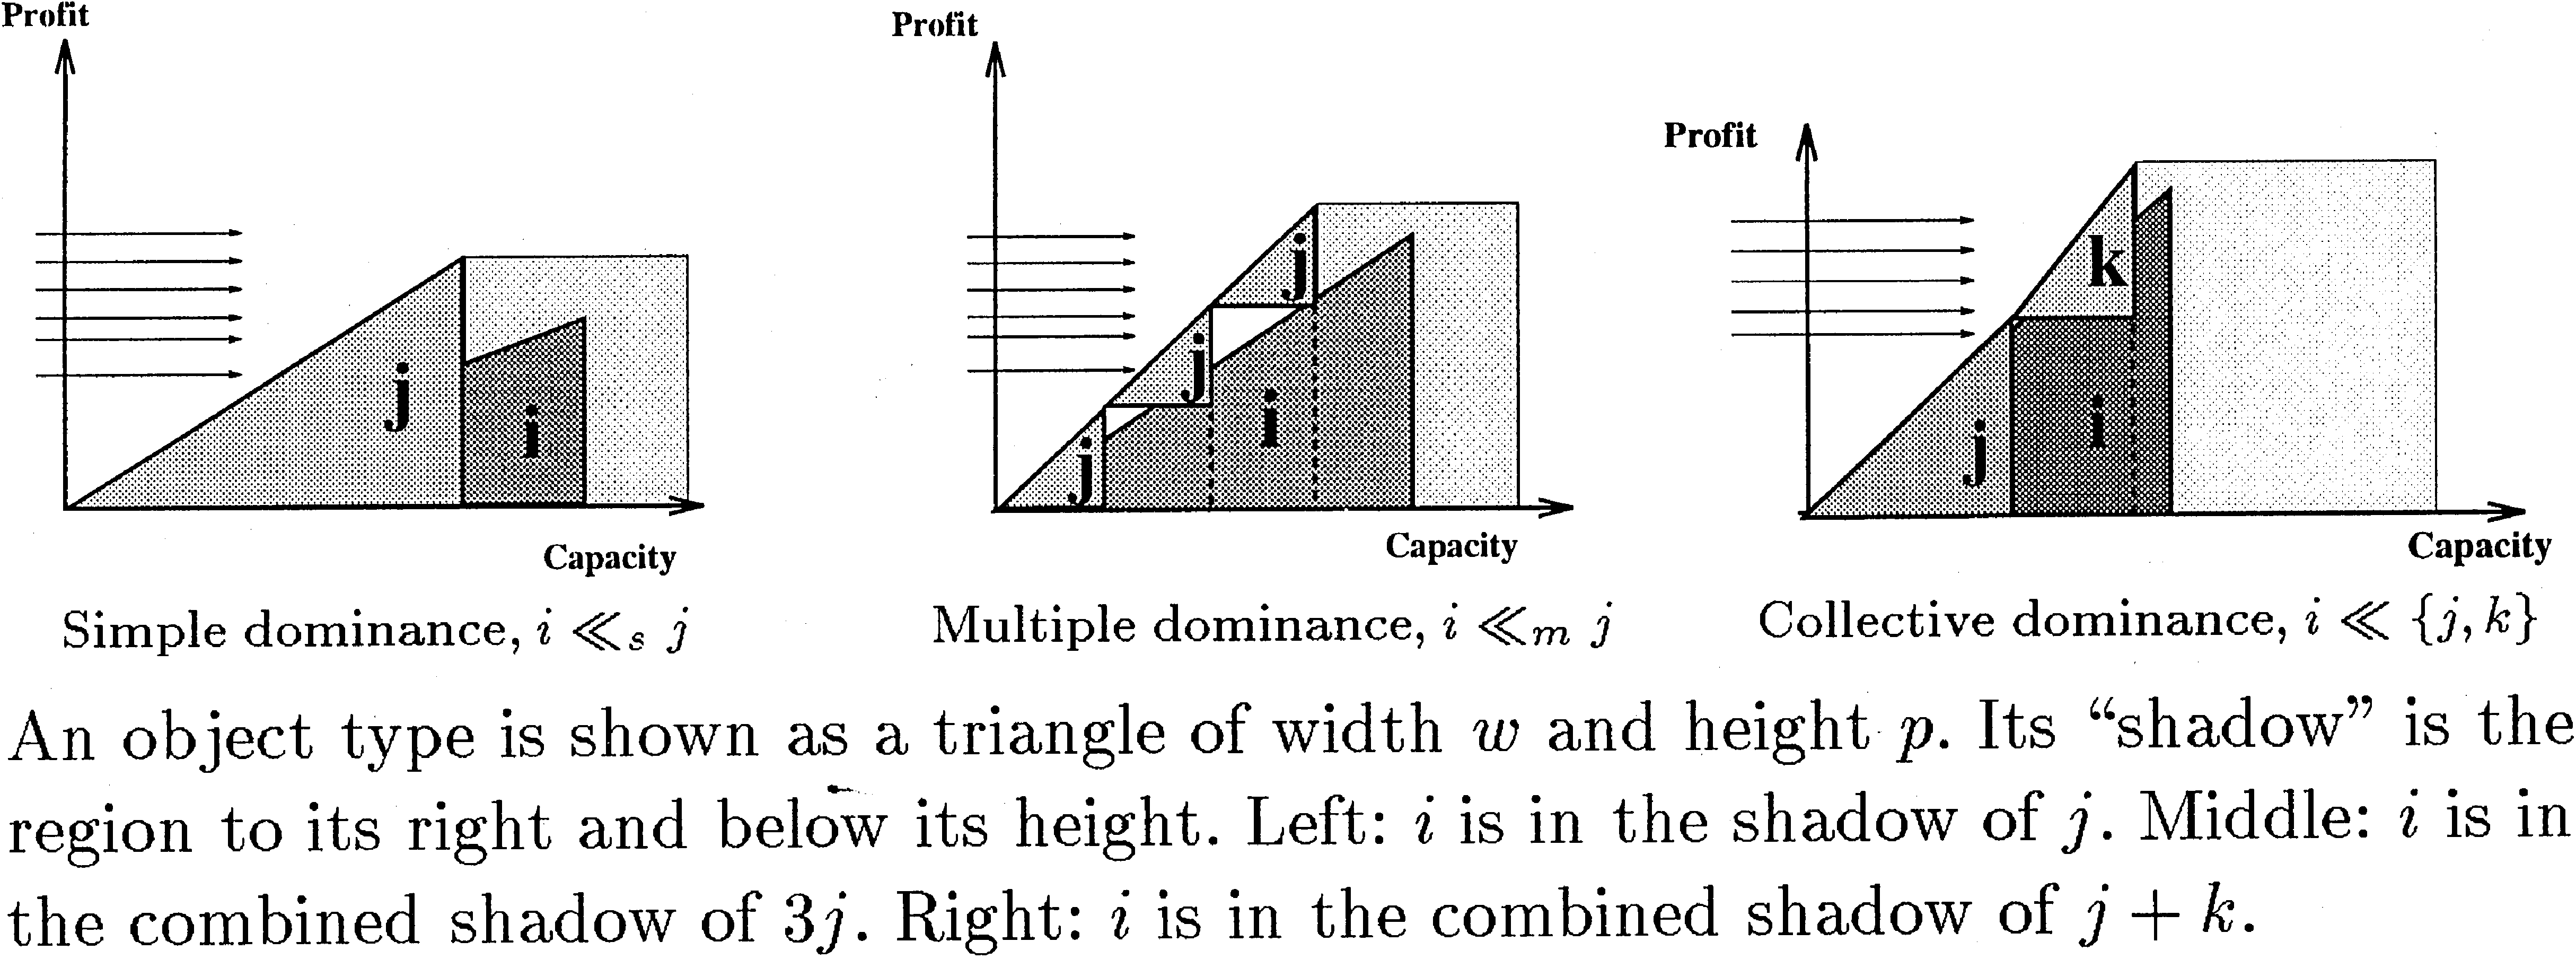
\includegraphics[width=1\textwidth]{smc_dominance}
  \caption{Classical graphic representation of the simple, multiple and threshold dominances. Source: \cite{eduk}. It is interesting to note that the triangle slope equals to the items efficiency, and that all points in the shaded area created by an item or solution triangle are dominated.}
\end{figure}

Given a solution~\(s\) composed of any items, and a solution \(t\) containing only two or more copies of an item \(j\), if \(w_s \leq w_t\) and \(p_s \geq p_t\), then it is said that solution \(s\) threshold dominates item \(j\).
This dominance relation is called \emph{threshold dominance}.
If~\(t\) is composed of~\(n\) copies of item~\(j\), then we know that we can disregard solutions with~\(n\) or more copies of item~\(j\) (as each group of~\(n\) copies of~\(j\) can be replaced by~\(s\) without loss to the value of the optimal solution).
Collective dominance can be seen as a special case of threshold dominance, where~\(n = 1\) (i.e. the dominated solution~\(t\) is a single item solution).

\begin{figure}
  \centering
  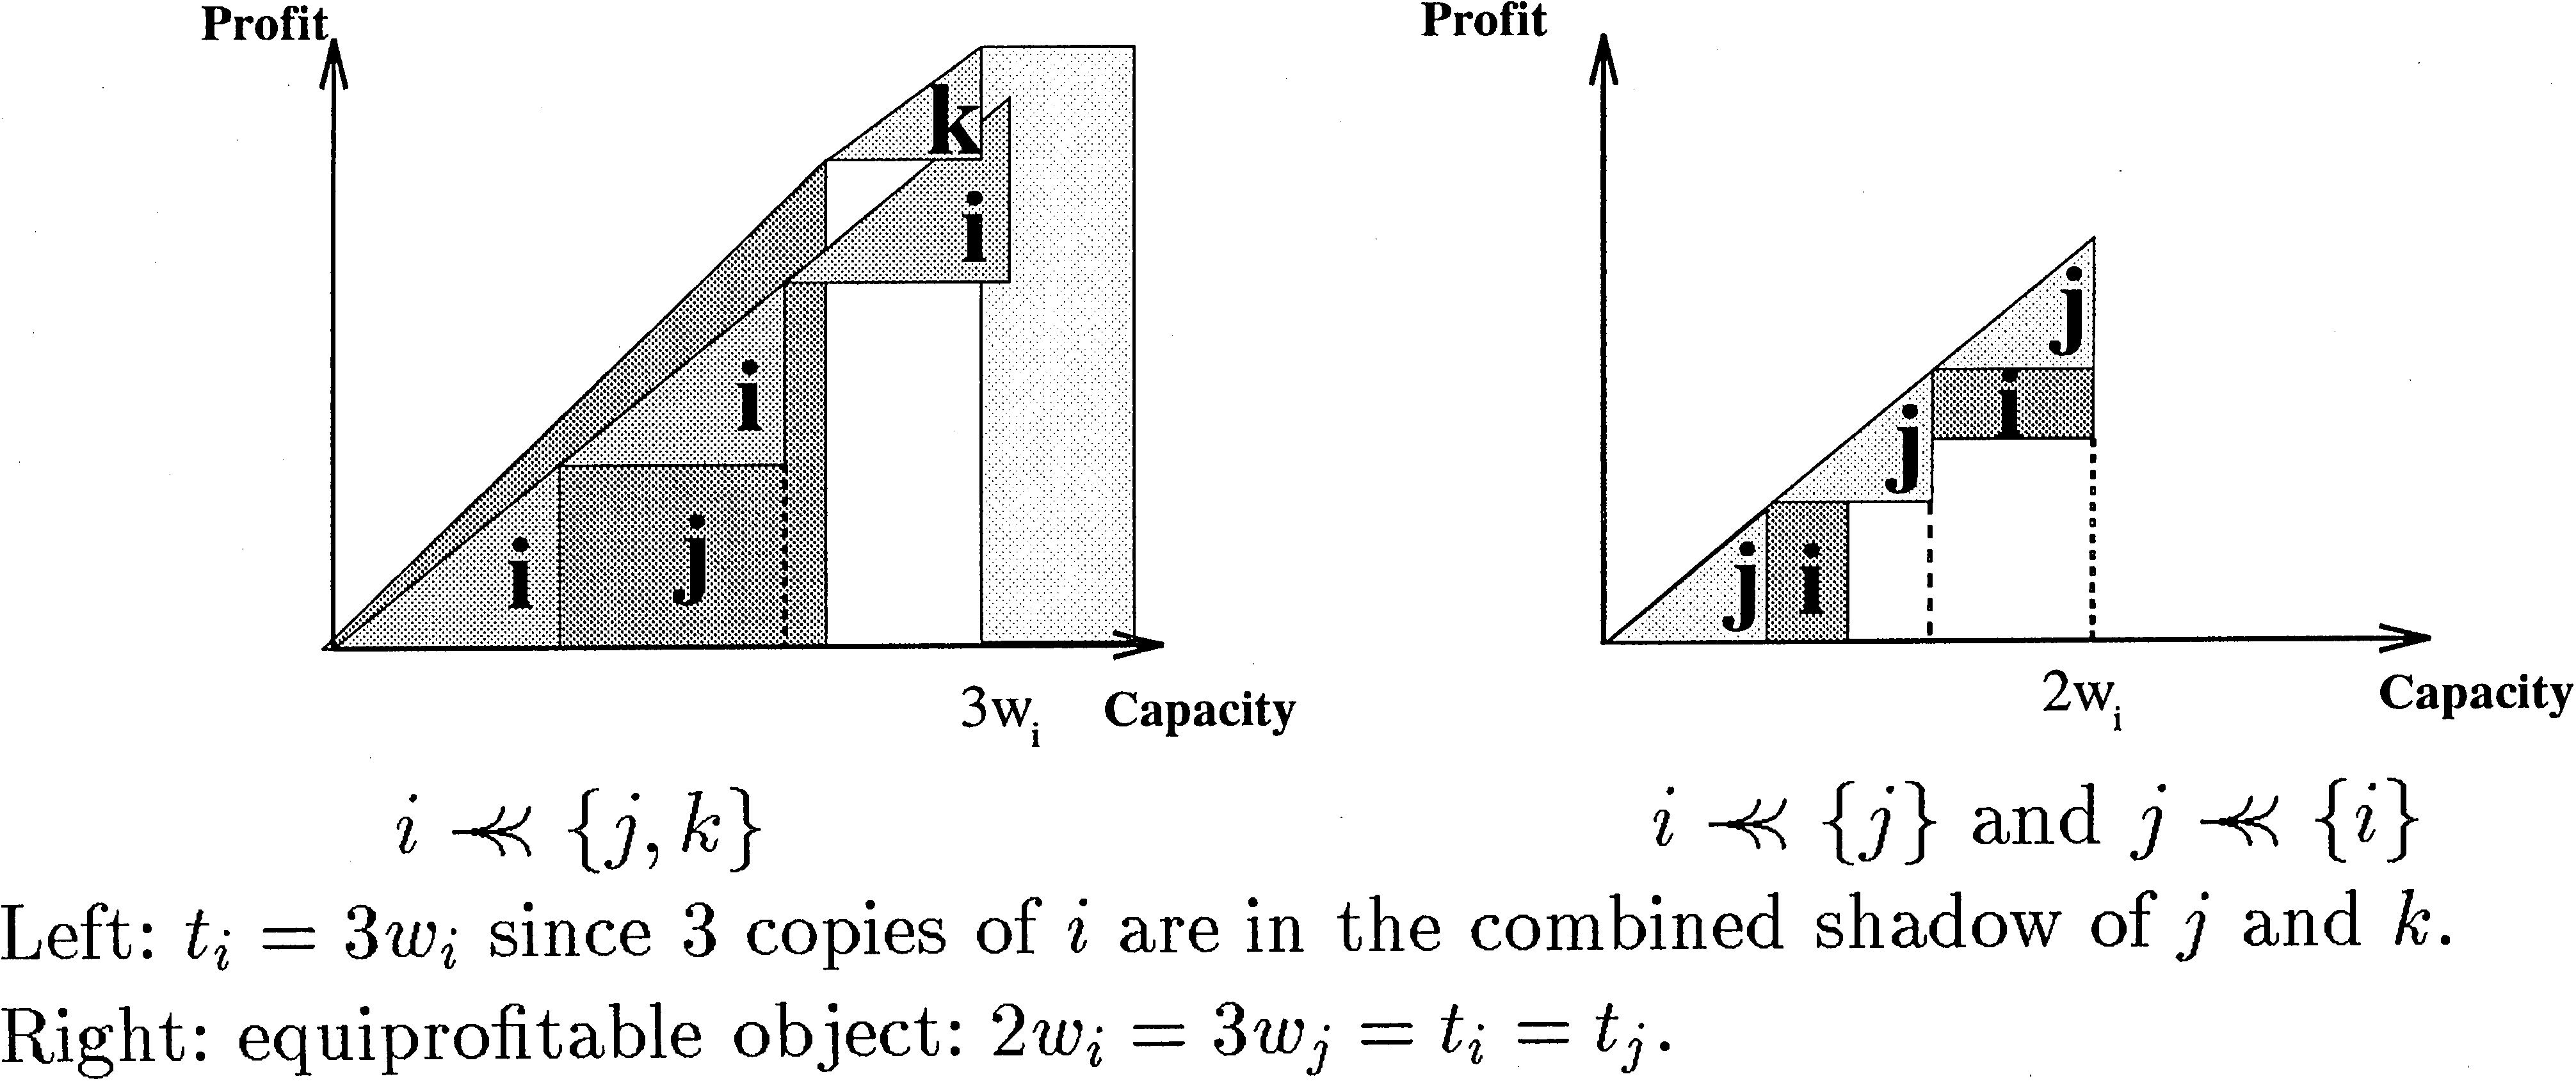
\includegraphics[width=1\textwidth]{threshold_dominance}
  \caption{Classical graphic representation of the threshold dominance. Source: \cite{eduk}. The \(t_i\) is the \emph{t}hreshold of item \(i\), i.e. the weight of the smallest solution composed only of copies of \(i\) that is dominated by another item/solution.}
\end{figure}

The simple and multiple dominances were deeply studied in the previous literature. 
Algorithms that remove all simple and multiple dominated items in~\(O(n^2)\), and heuristics with less complexity that do not guarantee removing all simple or multiple dominated items, were proposed, see~\cite{pisinger_thesis} for a good review on this subject.
On the other hand, the collective and threshold dominances seem too computationally expensive to be done in a preprocessing phase.
However, in the context of a Dynamic Programming (DP) algorithm, in which the optimal solutions of lower capacities can be reused to detect both collective and threshold dominances~\cite{pya}, these dominances are cheap to detect.

The Efficient Dynamic programming for the Unbounded Knapsack problem (EDUK) and the EDUK2 algorithms detect those four types of dominance relations~\cite{pya}.
In fact, threshold dominance was first proposed by the EDUK authors in~\cite{ukp_new_results}, and was a primary feature of the EDUK algorithm.
However, we will see that both algorithms seem to be dominated by algorithms that predate them by about forty years, as the \emph{ordered step-off} algorithm from~\cite{gg-66}, and its `improved version' from~\cite{green_improv}.
These two old algorithms did not directly apply any of the four types of dominance.

After examination, it becomes clear that these two old algorithms indirectly apply all four dominances.
By \emph{indirectly}, we means that, in the course of these algorithms execution, they eventually stop using dominated items to create new solutions, and that happens without testing items for each one of the four dominance relations previously explained.%, and then removing the dominated items from a global items list.
The approach used by these old algorithms is focused on solutions, not individual items.
Consequently, it would be more adequate to say that they make use of some sort of \emph{solution dominance}.
Ideally, given a solution~\(s\) and a solution~\(t\) (both \(s\) and \(t\) can be composed of any items), if \(w_s \leq w_t\) and \(p_s \geq p_t\), then an optimized algorithm could not generate any solutions that are a superset of~\(t\) (as the respective supersets of~\(s\) would dominate them anyway) without loss to the value of the optimal solution..
Such dominance relation would generalize all previous dominances, as the dominated items can be seen as single item solutions (or multiple item solutions, in the case of threshold dominance).

Those old algorithms do not apply this ideal solution dominance, but a weaker version of it.
This weaker version of solution dominance does not avoid generating every solution that is a superset from a dominated solution, but it can be implemented with almost no overhead.
As this is algorithm-specific, it will be further discussed in Section~\ref{sec:ukp5_sol_dom_expl}.

In this section, the concept of dominance was introduced by explaining four dominance relations found in the literature and proposing the concept of strong solution dominance.
In the literature, one of the definitions used for dominance is: ``Given an instance of UKP, relative to item types set~\(N\), item type~\(k \in N\) is dominated if the optimal solution value does not change when~\(k\) is removed from~\(N\).''~\cite[p. 100]{martello_book}.
This definition is consistent with simple, multiple, and collective dominance, but not with threshold dominance.
If an item is threshold dominated, it can still be present in all optimal solutions, it only cannot appear \(n\) or more times in all optimal solutions.
Solution dominance is not covered by this definition, as it is item-centric.
Finally, such broad definition of dominance does not give hints on how to design a procedure for removing the dominated items (without solving the instance), differently from the dominance relations.

\subsection{Periodicity and periodicity bounds}
\label{sec:periodicity}

% TODO: change y to y^{+} in the context of the capacity limit
%The UKP has an obvious periodic property that for every knapsack capacity that is a multiple of the best item's weight, the optimal solution for that knapsack capacity is~\(\frac{c}{w_b}\) copies of the best item (it's clearly the most efficient use that can be made of such capacity). The UKP has also a not-so-obvious and more interesting periodic property that states that:
The UKP has an interesting periodic property that can be stated the following way: for every set of item types, there exists a capacity~\(y^+\), for which every capacity~\(y'\) (\(y' > y^+\)) will have an optimal solution that is an optimal solution for capacity~\(y' - w_b\) with one more copy of the best item added.
In other words, after some capacity~\(y^+\), we can find optimal solutions simply by adding copies of the best item to optimal solutions of capacities~\(y^+\) and lower (all other items are not relevant anymore).
In the literature, this periodic property is called \emph{periodicity}.
It should be clear that if we knew~\(y^+\) beforehand, and~\(y^+ < c\), then we can solve the UKP for the capacity~\(y^{*} = c - \ceil{\frac{c - y^+}{w_b}}w_b\) and fill the gap between~\(y^{*}\) and~\(c\) with exactly~\(\frac{c - y^{*}}{w_b}\) copies of the best item (instead of solving the UKP for capacity~\(c\)).
%The focus of this section will be this second periodic property, that we will call simply by `periodicity'.

The periodicity is a direct consequence of the threshold dominance.
However, the periodicity was discovered much before the concept of threshold dominance.
For instance, periodicity was already described in~\cite{gg-66}.
As the concept of threshold dominance was already explained in this thesis, the author will use it to explain periodicity.

The threshold dominance property states that, if a solution~\(s\) dominates solution~\(t\), and~\(t\) contains only~\(n\) copies of the same item type~\(j\), then solutions with~\(n\) or more copies of~\(j\) can be be replaced by solutions using~\(s\) instead (without loss to the value of the optimal solution).
The periodicity property states that after some capacity~\(y^+\) we can obtain optimal solutions only by adding copies of the best item to the optimal solutions from capacities \(y^+\) or below (all other items are not relevant anymore).
The link between these two properties is that \emph{for a sufficiently large capacity, solutions composed of copies of the best item will threshold dominate solutions composed of copies of any other item}.

First, we will verify the truth of the statement above.
For any two positive integers~\(a\) and~\(b\) there will always exist at least one integer number that is divisible by both~\(a\) and~\(b\) (e.g.~\(a \times b\), or their \emph{least common multiple},~\(LCM(a, b)\)).
Therefore, for each non-best item~\(j\), there will exist a capacity value~\(y\) that it is divisible by both~\(w_b\) and~\(w_j\).
Given~\(m_j = \frac{y}{w_b}\) and~\(n_j = \frac{y}{w_j}\), and by the definition of best item, we have that~\(m_j \times p_b \geq n_j \times p_j\).
In other words, a solution composed only of~\(m_j\) copies of the best item will threshold dominate a solution composed only of~\(n_j\) copies of item~\(j\).

It is important to notice that, in the case of an instance in which all items have the same efficiency, the best item (that will have weight~\(w_{min}\) by definition) will threshold dominate each other item at the capacity that is the \emph{lowest common multiple} between their weights (as shown in the last paragraph).
However, if the best item~\(b\) is more efficient than the non-best item~\(j\) (which is more common), then a smaller solution~\(s\) composed only of copies of~\(b\) can be more profitable than a bigger solution~\(t\) composed only of copies of~\(j\).
The weights of the two solutions do not have to be the same.

Now, we explain how periodicity is a direct consequence of threshold dominance.
As we have seen, for each non-best item~\(j\), there will exist a positive integer~\(n_j\), in a way that solutions with~\(n_j\) copies of~\(j\) are dominated by solutions that use~\(m_j\) copies of~\(b\) instead.
We will assume that there exists a solution~\(u\) composed of~\(n_j - 1\) copies of each item~\(j\).
If another copy of any item~\(j\) is added to~\(u\), the resulting solution~\(u' = u~\cup~\{j\}\) could be replaced by another solution~\(v\) that contains no copies of~\(j\), and~\(m_j\) additional copies of~\(b\).
Any solution that weight more than solution~\(u\) has only two possibilities: it uses more copies of the best item; or it uses more than~\(n_j\) copies of some non-best item~\(j\).
In the last case, copies of~\(j\) can be replaced by copies of~\(b\) until the quantity of copies of~\(j\) is smaller than~\(n_j\).
Consequently, after the knapsack capacity~\(y'' = w_u\), adding copies of other items to a solution would be equal to adding copies of the best item (making any other item type except~\(b\) irrelevant).
Note that~\(y''\) is only an \emph{upper bound} on~\(y^+\), the value of~\(y^+\) can be smaller than~\(y''\), as the items that the best item threshold dominate, can themselves threshold dominates other items.

It's worth mentioning that computing the exact value of~\(y^+\) is a very expensive process that equals to solving the UKP for all capacities~\(y^+\) and lower while checking for threshold dominance.
The author do not know any algorithm for solving the UKP that computes the exact value of~\(y^+\) before starting to solve the UKP.
The algorithms compute an \emph{upper bound} on the~\(y^+\) capacity value, as the one presented in the previous paragraph, that was presented in~\cite[p.~215]{book_ukp_2004}.

An upper bound on~\(y^+\) is less valuable than~\(y^+\) itself, but it can be computed in a reasonable polynomial time, before starting the solving process.
If one algorithm checks for threshold dominance periodically, it can stop when all non-best items have been threshold dominated by the best item.
Such algorithm would not benefit much from computing an upper bound on the~\(y\) capacity value.
If this algorithm setup phase (e.g. allocating and initializing memory) is linear in the knapsack capacity~\(c\) and the upper bound on the~\(y\) capacity value is considerably smaller than \(c\), then the algorithm could benefit from the upper bound. 

There exist many proposed periodicity bounds, but some are time-consuming, as the~\(O(n^2)\) periodicity bound presented in~\cite{badbound1}. Others depend on specific instance characteristics to be tight, as the ones presented in~\cite{badbound2} and~\cite{pya}.
For reasons that will be made clear in the conclusions, the author did not found relevant to present a review on periodicity bounds in this work.
The UKP5 algorithm makes use of one simple periodicity bound, and it will be explained together with UKP5 in Section~\ref{sec:ukp5_periodicity}.


\chapter{Prior Work}
\label{sec:prior_work}

It is important to note that the name ``Unbounded Knapsack Problem'' is more recent than the problem itself.
To the best of our knowledge, this name was used for the first time in~\cite{mtu2}.
Earlier papers simply referred to `a' or `the' knapsack problem(s) the variant discussed was specified by the model presented in the paper.
An earlier paper from the same author tackled both the UKP and the BKP~\cite{mtu1} and called them, respectively, the General Unconstrained Knapsack Problem (GUKP) and General Constrained Knapsack Problem (GCKP).
In the paper, the adjective unidimensional was also used to characterize both variants.
More recently, the term `UKP' seems to be well accepted. Also, unidimensional is considered the default, and the term multi-dimensional is used to differ from it.
A researcher making a literature review about a specific variant of the knapsack problem should be aware of such caveat.

This literature review starts with~\cite{gg-61}, when the \emph{column generation} approach was proposed.
The main utility of the column generation approach was to avoid the existence of an exponential number of variables when solving the tightest linear programming model of BPP and CSP.
The relationship between the UKP and the BPP/CSP was already briefly described at Section~\ref{sec:motivation}, and its technical details will be described at Section~\ref{sec:csp_ukp_inst}.
The UKP is not solved, it is only said that ``the auxiliary problem will be of the integer programming variety, but of such a special type (the `knapsack' type) that it is solvable by several methods''~\cite[p.~2]{gg-61}.
Two years later, in~\cite{gg-63}, the authors proposed a specific algorithm for the UKP, and experiments solving BPP and CSP instances were executed.
Some findings of this experiments will be discussed in Sections~\ref{sec:csp_ukp_inst} and~\ref{sec:csp_experiments}.

%In this paper, the algorithm for UKP that was first described at~\cite{gg-63} is discussed more profoundly.
In~\cite{gg-66}, the one-dimensional and two-dimensional knapsack problems related to BPP and CSP were discussed.
The author of this thesis reinvented one algorithm from~\cite{gg-66} and published a paper about it, believing it was novel~\cite{sea2016}, thus, he apologizes to the academic and scientific community for such disregard.
Further information about the algorithms of~\cite{gg-66} and~\cite{sea2016} can be found in Section~\ref{sec:dp_algs}.
A small improvement over the algorithm of~\cite{gg-66} was proposed in~\cite{green_improv}.
The author implemented the improved algorithm and its results can be seen in Section~\ref{sec:pya_exp}.

The papers~\cite{cabot} and~\cite{turnpike} were published shortly after.
Both papers are behind a paywall and we did not have access to them.
However, the algorithm from~\cite{cabot} was compared indirectly by~\cite{mtu1} (that will be discussed in the followig pages).
The comparison showed that the algorithm from~\cite{cabot} was dominated by the algorithm proposed in~\cite{mtu1}.
In~\cite{green_improv}, it is implied that the proposed algorithm is an improvement over the algorithm from~\cite{turnpike}.
However, the author of this thesis believes that it would be interesting to implement and execute these algorithms on recent datasets.
In~\cite{mtu1}, empirical evidence was presented, but they used datasets considered to be small according to current standards.
They also used an items distribution that we have some reservations about (see Section~\ref{sec:martello_uncorrelated}). % TODO: probably a problem pointed out in Ritt's review
In~\cite{green_improv}, the claims are backed up by theoretical reasoning, nevertheless empirical evidence shown in Section~\ref{sec:pya_exp} revealed that the improvement had some unpredicted behavior over some instance datasets.
%The author thinks that revisiting such abandoned algorithms would be interesting, but it wasn't a priority in this work.

%This generated distortions and abandoned paradigms. The whole shift from dynamic programming methods to B\&B methods can be associated with the tests being made over ever-increasing instances; randomly generated with little or some correlation between profits and weights; and the use of naive dynamic programs; the shift of PYAsUKP to revisit dynamic programming can easily be correlated with the evolution of the artificial instances generated to be difficult to solve by B\&B while small (on capacity and number of items); the DP methods began to shine again, as the instances had small dimensions and a structure that made them hard to solve by B\&B but not so much by a good (non-naive) DP algorithm. The UKP5 is only the last part of this history.

%The paper ``A Finite Renewal Algorithm for the Knapsack and Turnpike Models'' and http://pubsonline.informs.org/doi/abs/10.1287/opre.18.2.306 were behind a paywall and the paper ``A better ...'' said to have a better algorithm anyway. 

%B\&B methods appear, and begin to claim that DP isn't efficient, they don't compare with the DP methods, only between each other, using some distributions and without motivation or real-world instances

% MTU1 and MTU2 papers:
In the 1970's, there was a shift of attention from the DP approach to the B\&B approach.
The first algorithms using this approach seem to be the Cabot's enumeration method~\cite{cabot} and the MTU1 algorithm~\cite{mtu1}.

MTU1 was proposed in~\cite{mtu1}, with the name of KP1 at the time (we will refer to this paper as the `MTU1 paper'). % old paper of MTU1 %To the author's knowledge, the MTU1 paper was the only paper to present experimental results comparing the B\&B and DP methods, before PYAsUKP paper, in 2009\cite{pya}.
Unfortunately, by current standards, the instances used in the comparison were very small (which is understandable considering the paper publishing date). 
The numbers of items used were 25, 50 and 100, for instance; the weights (and profits) had values between 11 and 110 (in the case of the profits, 120); the knapsack capacity was chosen between~\(0.2 \sum_{i \in n}{w_i}\) and~\(\sum_{i \in n}{w_i}\); the distributions used were uncorrelated and weakly correlated (\(p_i = w_i + \alpha\), where~\(\alpha\) was randomly chosen from -10 and 10 following an uniform distribution).

The comparison presented in~\cite{mtu1} was between KP1 (MTU1), the dynamic programming algorithm called `periodic step-off' from~\cite{gg-66}, that we will call G.G. for short, and two B\&B algorithms for the 0-1 KP (for which the UKP instances were transformed in 0-1 KP instances).
The best results were from MTU1, and the second best from the G.G. algorithm.
However, the instances were too small to draw strong conclusions, and the relative difference between G.G. and MTU1 average times was not even one order of magnitude apart.
The G.G. algorithm was about four times slower than MTU1 in the instances with~\(n = 25\); about two or three times slower in the instances with~\(n = 50\); and less than two times slower in instances with~\(n = 100\).
This trend could indicate that for big instances, the G.G. algorithm would have better times than MTU1 (e.g. the G.G. algorithm could have a costly initialization process but a better average-case asymptotic complexity).

%The MTU1 paper~\cite{gen_uni_knap_prob} also makes an indirect comparison with Cabot's B\&B algorithm. The MTU1 paper uses the dataset described in Cabot's paper~\cite{cabot}, and arrives at the conclusion Cabot's algorithm is clearly dominated by MTU1. The instance dimensions are only a little different to the ones used in their experiment described above (number of items up to 80, only uncorrelated distribution).

The experiments described above were used by the authors on another paper to state that ``The most efficient algorithms for the exact solution of the UKP [...] consist of two main steps: Step 1. Sort the item types according to (5). Step 2. Find the optimal solution through branch-and-bound.''~\cite{mtu2}. This comment established B\&B as most efficient approach for the UKP.
The paper introduced the MTU2 algorithm (and the author will refer to it as the `MTU2 paper').

The MTU2 algorithm was designed for large instances (up to 250,000 items).
Only sorting the items list was already computationally expensive for the period, and the solutions often involved only the most efficient items.
The MTU2 main feature was grouping and sorting only the~\(k = max(100, \frac{n}{100})\) most efficient items, and calling MTU1 over them.
The UKP instance consisting of this reduced items list and the original knapsack capacity was called `tentative core problem'.
If the optimal solution of the tentative core problem was proven to be optimal for the original problem, the algorithm stopped.
Otherwise, the optimal solution of the tentative core problem was used as a lower bound to remove dominated items.
After this, the~\(k\) most efficient items outside the tentative core problem were added to it, restarting the process. 

The algorithms comparison included only MTU1 and MTU2.
The datasets used in the paper were large, but artificial and abundant in dominated items.
A more detailed analysis of one of the datasets and the experiment setting is available in Section~\ref{sec:martello_uncorrelated}.
The MTU2 was clearly the best algorithm for the chosen datasets.

MTU2 was adopted by the subsequent works as the baseline for testing new algorithms for the UKP.
We believe this happened due to many factors, such as: the code of MTU2 was freely available; the algorithm was well and thoroughly explained in Martello and Toth's publications; it presented empirical evidence of dominating other methods and, consequently, comparing with it would remove the necessity of comparing to many other algorithms; the description of MTU2 stated that it was designed for large instances.
However, MTU2 does not completely dominate MTU1, it simply was better for the chosen instances (that were chosen with the purpose of evidencing this).
Instances in which the MTU2 needs to repeat the process of adding items to the tentative core problem many times can be more easily solved by MTU1 than by MTU2.
Unfortunately, the works that followed chose to compare their algorithms only against MTU2.

EDUK (\emph{Efficient Dynamic programming for the Unbounded Knapsack problem}), a novel DP algorithm for the UKP, was proposed in a conference paper~\cite{ukp_new_results} and then presented in a journal paper~\cite{eduk}.
EDUK is very different from the previous DP algorithms, and its main features are the application of threshold dominance (proposed in the same paper), and the use of a sparse representation of the iteration domain.
This last feature was implemented by using lazy lists, mainly because EDUK was implemented in the functional language OCaml.
EDUK is strongly based on the ideas first discussed in~\cite{algo_tech_cut}.

In~\cite{eduk}, the authors criticize the item distributions used in previous papers, especially the uncorrelated distribution.
The author of this thesis agrees with this criticism, further discussion can be found in Section~\ref{sec:inst_uncorrelated}.
However, the solution given for this problem were new datasets of artificial instances.
The new datasets do not have simple dominated items, or small efficient items, as the previous datasets, and one of them does not even have any collective dominated items.
The change in the choice of items distributions benefits DP methods (and consequently EDUK), which are better suited for such kind of instances.
When the new datasets are used, the comparison between MTU2 and EDUK shows that the average times of MTU2 are strongly dominated by the ones of EDUK.

The weakly and strongly correlated distributions are also used in \cite{eduk}, but varying the value of~\(w_{min}\).
For those instances, MTU2 dominates EDUK when the weight of the smallest item is close to one, but MTU2 times grow much faster than EDUK times when~\(w_{min}\) is increased.
Only one comparison is made against another DP algorithm.
The DP algorithm used seems to be a na{\"i}ve DP algorithm with a preprocessing phase that removes simple dominance.
The comparison uses a completely different dataset of small instances, in an effort to take into account real-world applications of the UKP, as the ones provenient from solving BPP and CSP with column generation.
The average run times in this comparison are smaller than 0.1 seconds, and the difference between the average times of EDUK and the naive DP are about 20\% (with EDUK being faster).

EDUK2 is an improvement of EDUK proposed in~\cite{pya}.
The main improvement brought up by EDUK2 is the hybridization of EDUK with the B\&B approach.
A B\&B preprocessing phase was added to EDUK.
If it solves the instance using less than a parametrized number of nodes, then EDUK is never executed; otherwise, the bounds computed in the B\&B phase are used to reduce the number of items before EDUK execution and in intervals during its execution.
The paper also proposes a new bound for a subset of the strongly correlated instances (the SAW instances), which that is the tightest bound known for such instances.
Comparisons are performed with EDUK and MTU2.
EDUK2 is clearly the winner, but the average solution times of the methods are few seconds, or less than a second.
The experiments are then remade using the same distributions with larger coefficients.
MTU2 has integer overflow problems and is left out of the comparison.
Between EDUK and EDUK2, EDUK2 has the best results, as expected. 

Both~\cite{eduk} and~\cite{pya} cite~\cite{babayev}, which presents an algorithm for solving the UKP using the Consistency Approach (CA).
The algorithm described in~\cite{babayev} was tested against MTU2 and had better times, but the instances used in the experiment make it difficult to have an idea of what would be its performance using more recent datasets (see Section~\ref{sec:babayev_uncorrelated} for further discussion).
The CA was already discussed in~\cite{on_equivalent_greenberg}.
However, the algorithm proposed in~\cite{babayev} considered performance as a priority, different from previous works that treated applying CA to the UKP as an interesting theoretical problem.
As the authors of~\cite{eduk} and~\cite{pya}, we tried to obtain a copy of the code from the authors of~\cite{babayev}, but did not obtain success.
The author of this thesis suggests the implementation and comparison of this algorithm as a future work.

Before ending this literature review, we would like to discuss the chapters about the UKP in the following textbooks:~\cite{tchu} and~\cite{garfinkel}.
Those textbooks are especially relevant because they are cited by many of the papers presented at this section.
The chapter about the UKP in~\cite[p.~311]{tchu} has a good introduction about the problem, the simplest DP method for solving it, and the basics of the periodicity.

The chapter about the UKP in~\cite[p.~214]{garfinkel} has an extensive bibliographical review of the works about the UKP that predates it (1972), which is very relevant as the name `UKP' was only established some years later.
%The chapter also discusses in depth many of the approaches used to solve the UKP in that period, yet making heavy use of mathematical notation.
In Section~\ref{sec:gg_algs}, we discuss a limitation of the review proposed in that chapter.
%In the Section 6.4 of the book, a DP algorithm is presented as the last of a series of improvements over the naive DP algorithm. However, if we check the chapter notes, there's the comment ``6.4: The recursion of this section is based on Gilmore and Gomory (1966). See Exercise 21 for a variation that will be more efficient for some data sets.''. The algorithm presented in section 6.4 was a version of the algorithm in~\cite{gg-66} with \emph{some} of its main optimizations removed, and in exercise 21 is expected of the reader to recreate \emph{one} of those optimizations based in hints given at the exercise. The author of this thesis believes that this fact can have been unnoticed by previous authors that cited the work. The book didn't featured the exercises' answers. % TODO XXX COPY THIS PARAGRAPH TO ALGORITHMS SECTION

% A LITTLE OF CSP HISTORY TOO
%\section{Cutting Stock}

% BLOCKQUOTE BELOW
% This corresponds to widely-used practices and general beliefs expressed in the literature. Usually, in the context of an LP- based branch-and-bound algorithm, where the LP relaxation is solved using column generation, cutting planes are carefully selected in order to avoid the destruction of the structure of the pricing problem. This viewpoint is shared by numerous authors. Barnhart, Hane, and Vance [BHV00], for example, mention as one of the main contributions of their branch-and-price-and-cut algorithm ``a pricing problem that does not change even as cuts are added, and similarly, a separation algorithm that does not change even as columns are added.'' (BELOV, page 3)

%About the pricing problem with cuts. ``It is much more difficult than the linear knapsack problem for column generation arising when no cuts are added in the LP.'' (BELOV, page 26)

% The paragraph below is only about 2D-2CP?
%``The general-purpose cuts considered in this work make the pricing problem extremely complicated and much implementation effort is required. The question arises, whether any other classes of cuts, which do not complicate the pricing problem, e.g., cover inequalities in 2D-2CP, can provide a comparable contribution.'' (p.~46)

% maybe this goes in another section
%	timeline: DP -> huge random instances -> B\&B is better (no empiric evidence) -> instances that are hard for B\&B (linear distribution) -> PYAsUKP is better than B\&B in instances designed to be hard to solve by it (in fact any DP non-naive DP solution would have results better than B\&B methods only, like MTU1 and MTU2). also, using MTU2 instead of MTU1 shows a lack of understanding of the methods. MTU2 was developed for very large random instances, not for relatively small and hard (distribution-wise) instances


% MAYBE ADD
% The subject that I (Henrique Becker) am studying (at the year of 2015/2016) is the exact resolution of the UKP (unbounded knapsack problem) with the objective of solving the subproblems generated by the column generation approach of solving BPP/CSP (Bin Packing Problem and Cutting Stock Problem). The paper "An Improved Knapsack Solver for Column Generation" (2013, Klaus Jansen and Stefan Kraft) seemed (by the title) to be relevant to my studies. However, the paper presents a variant of the UKP, the UKPIP (the Unbounded Knapsack Problems with Inversely Proportional Profits) that's a subproblem of the Variable-Sized Bin Packing (VBP) that's a generalization of the BPP when there's the possibility of choosing between many bin sizes (on the classical BPP there's one fixed bin size for instance). The UKIPIP is a generalization of the UKP, in the sense that it allows for choosing between many knapsack sizes, and when restricted to only one knapsack size it's equivalent to the UKP. Yet, when there's many knapsack sizes to choose from, the same solution in different knapsacks will yield a diferent profit value, as the profit value of the items is scaled by the knapsack size (the smaller the knapsack size, the bigger the profit value for the same solution); and the solution is a multiset of items and the one knapsack choosen to store these items. The paper seems to focus on approximation methods to solve the UKPIP and the other two variants of it (the bounded one, BKPIP and the 0-1 one, 0-1 KPIP). So the subject of the paper (approximation algorithms for a variant of the UKP as subproblem of a variant of the BPP) is outside our area of interest (exact algorithms for the classical UKP as a subproblem of the classical BPP).

\chapter{The instance classes}

%final
If the author of this work could suggest one single thing to be improved in the future works about UKP, it would be the selection of the instances.

%working
The UKP is a variation of the classic knapsack problem, with the difference that an unbounded number of each item is available.

The study of the UKP has fallen in one of the pitfalls described by David Johnson in his guide to 

%pending
the ukp seems like a problem that should have many applications, but <CITE PYAsUKP 'are hard to find'>
the most classical real-world use of the problem is the unidimensional cutting stock problem 
	explain the problem
	explain how branch and price can be used to solve the problem
	cite gilmore and gomory (and brevily point that UKP5 and ordered step-off are very similar, more will be said in the algorithms section)
point error in the article, the pure UKP can only be used to solve the root node of the cutting stock exact continuous relaxation
the best solver don't use UKP anymore at all, but one of the good solvers use it, and repoted that in some cases, about 70\% of the processing is done at the root node

the use of artificial instances was already strongly crticized in the past
the reasons for their use is the possibility of generating many instances, of many sizes (what allows for examinating the growth of the time with the growth of the instance)
	This is specially interesting for UKP because it's one of the easiest NP-Hard problems, so big instances or hard instances have to be used to get high execution times, small execution times are too much affected by variance
	yet, artificial instances should not be used at all, if there's no guarantee that the growth/time/results will translate for real world instances (i.e. artificial instances should follow )

	The paper are the hard knapsack problems shows that even for 0-1 knapsack instances (that are by default harder than UKP instances), the instances used were easy to solve


The major problem with an experimental analysis of the UKP solving methods over artificial instances is that the different solving approaches are affected by the items distributions (i.e. some methods are the best for some for some distributions and the worst for others). Consequently, the results aren't useful for someone that wants to tackle real world UKP instances, unless some artificial instance distribution ends up modelling the 

TODO: The use of testbeds is overrated?

We have already pointed (TODO: refer to timeline) that the choices of item distributions on the generation of artificial instances in the previous literature has defined what was considered the best algorithm. I have written two sections of this chapter to further illustrate this point. Those are sections are (TODO: refer to) uncorrelated instances, and the second is the BREQD instances. The former points (TODO: list things pointed in uncorrelated instances); the latter presents a new instance distribution, that's easy to solve by B\&B methods and hard to solve by DP methods (some experimental results over this classes of instances will be presented at TODO: refer).

\section{Uncorrelated Random Coeficients Instances}

In this work, the expression `uncorrelated instances' will be used to refer to a family of UKP instances where the weight and the profit of an item have no correlation. The most common way for generating those uncorrelated instances is generating a value between \(w_{min}\) and \(w_{max}\) for the weight, and a value between \(p_{min}\) and \(p_{max}\) for the profit, for each of the \(n\) items of the instance using a (pseudo-)random number generator with an uniform distribution. %Uncorrelated instances can be generated using a (pseudo-)random number generator to generate \(n\) numbers between \(w_{min}\) and \(w_{max}\), and another \(n\) numbers between \(p_{min}\) and \(p_{max}\). Sorting both arrays will give (TODO: refer to realistic instances), that is another instance type. Uncorrelated instances 

PUTS IMAGE
\begin{figure}
    \caption{An uncorrelated instance generated with \(n = 100\), \(w_{min} = 1\), \(w_{min} = 1000\), \(p_{min} = 1\), and \(p_{max} = 1000\).}
    \begin{center}
    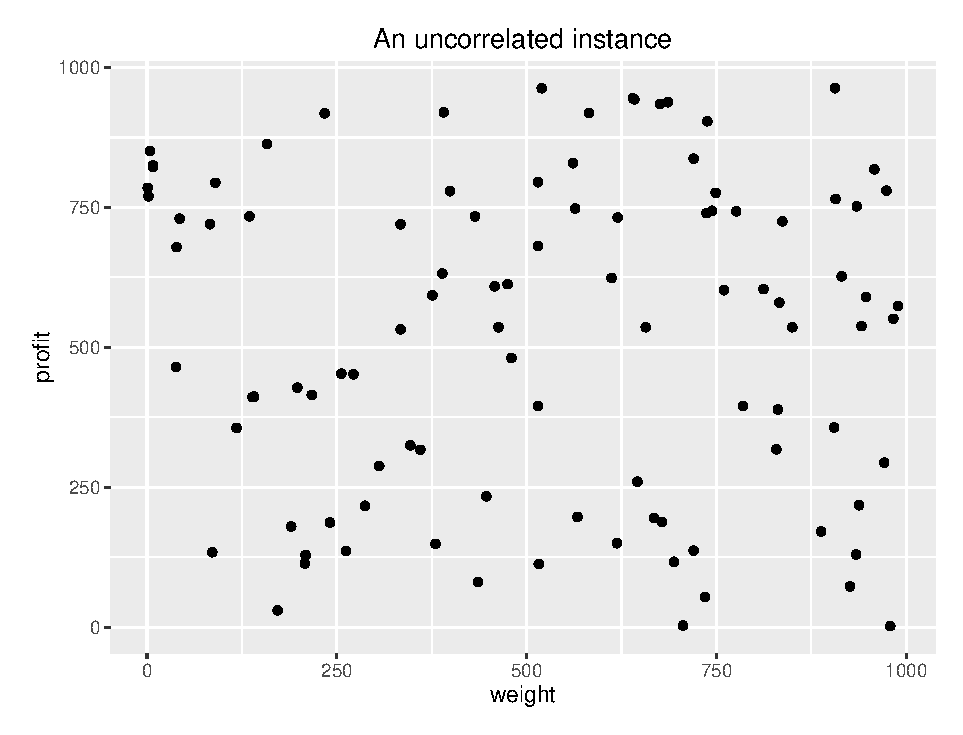
\includegraphics[scale=1]{uncorrelated.eps}
    \end{center}
    \legend{Source: the author.}
    \label{fig:uncorrelated_example}
\end{figure}

Expose why they are uninteresting: we do not know if they model any real world instance; it's a simple matter of running a good polynomial simple/multiple dominance algorithm first, or using MTU2 that was developed for this purpose. Increasing values of \(n\) increase the time taken by MTU2 or dominance removal in a polynomial fashion. The NP-hard part of the problem, that is finding an optimal solution between non-dominated items don't grow with \(n\). %(sorting or the \(O(n^2)\) dominance algorithms).

\section{Bottom Right Ellipse Quadrant Instances}

The Bottom Right Ellipse Quadrant Instances (`BREQ instances', for short) is a new UKP instance item distribution proposed by the author in this work. This instance distribution was created to illustrate that different item distributions favor different solution approaches and, therefore, the choice of instances (or specifically, their item distribution) defines what is considered the `best algorithm'.

Distributions that are easy to solve by the DP approach and hard to solve by the B\&B approach are common in the literature. This distribution has the opposite characteristic, it is hard to solve by DP and easy to solve by B\&B. It's important to point that this is an artificially generated distribution that don't model any real world instances (that the author have knowledge). The author discourages the use and study of such artificial instances, and created this distribution only as a tool to demonstrate that isn't hard to create a distribution that benefits a solving approach over another. It's the author's opinion that research should focus on real-world instances and/or artificially generated instances that clearly model real world instances.

The name given to this distribution is derived from the fact that, when plotted on a graph, the items show the form of a quarter of ellipse (specifically, the bottom right quadrant). All items in such distribution respect the following equation: \(p_i = p_{max} - \floor[\big]{\sqrt{p_{max}^2 - (w_i^2 \times \frac{p_{max}}{w_{max}}^2)}}\)\footnote{In this context, \(w_{max}\) and \(p_{max}\) define the quadrant top right corner, i.e. the possible maximum value for an item's weight and profit, an item with those exact values doesn't need to exist in a BREQ instance. The rounding down in the formulae can be dropped if the profit is a real number and not an integer.}. A natural consequence of this distribution shape is that the item profit grows quadratically with the item weight. This leads to the inexistance of simple, multiple and collective dominance\footnote{In truth, if the profit is integer, the smallest items can display some of those three dominances because the profit precision loss by rounding, but this is of little relevance and can be safely ignored for most purposes. If profit is an infinite precision real, the statement has no exceptions.}. In other words, for any multiset of items \(s\) and any single item \(i\) (with respective weigths \(w_s\) and \(w_t\), and respective profits \(p_t\) and \(p_i\)), if \(w_s \leq w_i\) then \(p_s < p_i\).

On the other hand, threshold dominance is very common in this instance type. With exception of the best item, any item of any instance (of any distribution) will always be threshold dominated at some capacity. However, in many instances the knapsack capacity is smaller than those threshold values and therefore the threshold dominance isn't applied or relevant. On BREQ instances, as a consequence of the quadratic profit growth, an optimal solution will never include the item \(i\) two or more times if there's an item \(j\) such as that \(\sqrt{2} \times w_i < w_j \leq 2 \times w_i\); so each item have a good probability of being threshold dominated before the second use. 

The solutions of BREQ instances will often contain the maximum number of copies of the largest item (that is also the most profitable, and the most efficient) allowed by the instance capacity. Any gap left will probably be filled by the heaviest item that fits the gap, with this process repeated until no item fits the gap left. A greedy heuristic procedure that followed those steps would probably yield an optimal solution. However, this is not always the case\footnote{A counter-example follows: consider an instance with \(n = 4\), \(c = 512\), \(w_1 = 384\), \(p_1 = 2774\), \(w_2 = 383\), \(p_2 = 2756\), \(w_3 = 129\), \(p_3 = 265\), \(w_4 = 32\) and \(p_4 = 17\); the optimal solution don't use the best item (\(w_1, p_1\)); the best solution when using the best item has a profit value of \(2842 = 2774 + 4\times17\) (weight \(512 = 384 + 4\times32\)) while the best solution when using the second most efficient item has the optimal profit value of \(3021 = 2756 + 265\) (weight \(512 = 383 + 129\)). In this case, between two solutions with the same weight, the one with the best item isn't the best one. The weight and profit values of this example follow the a BREQ distribution with \(w_{max} = 512\) and \(p_{max} = 8192\).}.

Our objective is not explore this distribution and its behaviour with different paremeters. Therefore, from now on we will refer only to instances with \(p_{min} = w_{min} = 1\) and \(w_{max} = c\). 

\section{Uncorrelated Random Coeficients Instances}

\section{Chung}
% TEX COPIED FROM SEA 2016 article, CHANGE AND AMPLIFY

\section{PYAsUKP instances}

This section will discuss the instance sets used in~\cite{pya}.
The distributions used by the instances weren't novel, but a 
Those instance sets were artificially generated with the purpose of being ``hard to solve'', what means a different thing for each one of them.


The same tool was used to generate the datasets (PYAsUKP), and the same parameters were used, otherwise noted the contrary. 
In Subsection 5.1.1 \emph{Known ``hard'' instances} of~\cite{pya} some sets of easy instances are used to allow comparison with MTU2. 
However, the authors reported integer overflow problems with MTU2 on harder instances. 
With exception of the subset-sum dataset, all datasets have a similar harder set (Subsection 5.2.1 \emph{New hard UKP instances}~\cite{pya}).
Thus, we considered in the runs only the harder ones. 
Each instance has a random capacity value within intervals shown in Table~\ref{tab:times}. 
The PYAsUKP parameters \mbox{\emph{-wmin \(w_{min}\) -cap c -n \textbf{n}}} were used in all instances generation. 
%When we found a discrepancy between the formula presented in \cite{pya} and the PYAsUKP code, or generated instances, we opted for changing the formula based on the observed behavior. 
%As our knowledge of OCaml is limited, we cannot guarantee that the formula presented here is a perfect match for the code; but, based by the generated instances, we believe it to be correct to a good extent.
We found some small discrepancies between the formulas presented in~\cite{pya} and the ones used in PYAsUKP code.
We opted for using the ones from  PYAsUKP code, and they are presented below.

\subsubsection{Subset-Sum}\label{sec:subsetsum}
Instances generated with \(p_i = w_i = rand(w_{min}, w_{max})\). 
The majority of the subset-sum instances used in \cite{pya} were solved on less than a centisecond in our experiments. 
This makes it easy to have imprecise measuring. 
Because of this, in this paper, we use a similar dataset, but with each parameter multiplied by ten. 
Therefore, we generated 10 instances for each possible combination of: \(w_{min} \in \{10^3, 5\times10^3, 10^4, 5\times10^4, 10^5\}\); \(w_{max} \in \{5\times10^5, 10^6\}\) and \(n \in \{10^3, 2\times10^3, 5\times10^3, 10^4\}\), totaling 400 instances. We do not discriminate each combination in~Table \ref{tab:times} for brevity. The PYAsUKP \emph{-form ss -wmax \(w_{max}\)} parameters were used.

\subsubsection{Strong Correlation}
Instances generated using the following formula: \(w_i = w_{min} + i - 1\) and \(p_i = w_i + \alpha\), for a given \(w_{min}\) and \(\alpha\).  Note that, except by the random capacity, all instances with the same \(\alpha\), \(\mathbf{n}\), and \(w_{min}\) combination are equal. The formula doesn't rely on random numbers. The PYAsUKP \emph{-form chung -step \(\alpha\) } parameters were used.

\subsubsection{Postponed Periodicity}
This family of instances is generated by the following method: \textbf{n} distinct weights are generated with \(rand(w_{min}, w_{max})\) and then sorted by increasing order; \(p_1 = w_1 + rand(1, 500)\); and \(\forall i \in [2, n].~p_i = p_{i-1} + rand(1, 125)\). The \(w_{max}\) is computed as \(10\overline{n}\). The PYAsUKP \emph{-form nsds2 -step 500 -wmax \(w_{max}\)} parameters were used.

\subsubsection{No Collective Dominance}
This family of instances is generated by the following method: \textbf{n} distinct weights are generated with \(rand(w_{min}, w_{max})\) and then sorted by increasing order; \(p_1 = p_{min} + rand(0, 49)\); and \(\forall i \in [2, n].~p_i = \lfloor w_i \times ((p_{i-1}/w_{i-1}) + 0.01)\rfloor + rand(1, 10)\). The given values are: \(w_{min} = p_{min} = \mathbf{n}\) and \(w_{max} = 10\overline{n}\). The PYAsUKP \emph{-form hi -pmin \(p_{min}\) -wmax \(w_{max}\)} parameters were used.

\subsubsection{SAW}
This family of instances is generated by the following method: generate \textbf{n} random weights between \(w_{min}\) and \(w_{max} = 1\overline{n}\) with the following property: \(\forall i \in [2, n].~w_i~mod~w_1 > 0\) (\(w_1\) is the smallest weight); sort by increasing order; then \(p_1 = w_1 + \alpha\) where \(\alpha = rand(1,5)\), and \(\forall i \in [2, n].~p_i = rand(l_i, u_i)\) where \(l_i = max(p_{i-1}, q_i)\), \(u_i = q_i + m_i\), \(q_i = p_1 \times \lfloor w_i / w_1 \rfloor \), and \(m_i = w_i~mod~w_1\). The PYAsUKP \emph{-form saw -step \(\alpha\) -wmax \(w_{max}\)} parameters were used.

% maybe this goes in another section
	timeline: DP -> huge random instances -> B\&B is better (no empiric evidence) -> instances that are hard for B\&B (linear distribution) -> PYAsUKP is better than B\&B in instances designed to be hard to solve by it (in fact any DP non-naive DP solution would have results better than B\&B methods only, like MTU1 and MTU2). also, using MTU2 instead of MTU1 shows a lack of understanding of the methods. MTU2 was developed for very large random instances, not for relatively small and hard (distribution-wise) instances


\chapter{Approaches and algorithms}
\label{sec:app_and_alg}

In this chapter, some approaches and algorithms for solving the UKP will be discussed.
The objectives of this chapter are: to present relevant details that did not fit in the literature review; to further develop what was said in the last section, about some approaches favoring some item distributions; to give readers some base to understand the results of the experiments (Section~\ref{sec:exp_and_res}); and to explain the concept of solution dominance, mentioned in Section~\ref{sec:dom_rel}.
The objective is not to present an exhaustive list of approaches and algorithms.

%Two techniques are often used for solving UKP: dynamic programming (DP)~\cite{eduk},~\cite[p. 214]{garfinkel},~\cite[p. 311]{tchu} and branch and bound (B\&B)~\cite{mtu2}. 
%The DP approach has a stable pseudo-polynomial time algorithm linear on the capacity and number of items. 
%The B\&B approach can be less stable. 
%It can be faster than DP on instances with some characteristics, such as when the remainder of the division between the weight of the best item by the capacity is small; or the items have a big efficiency variance. Nonetheless, B\&B has always the risk of an exponential time worst case.
% The state-of-the-art solver for the UKP, introduced by~\cite{pya}, is a hybrid solver that combines DP and B\&B. 
%It tries to solve the problem by B\&B, and if this fails to solve the problem quickly, it switches to DP using some data gathered by the B\&B to speed up the process. 
%The solver's name is PYAsUKP, and it is an implementation of the EDUK2 algorithm.

\section{Conversion to other KP variants}

In Section~\ref{sec:introduction}, it was pointed out that the UKP can be seen as a special case of BKP where, for each item type~\(i\), there are at least~\(\floor{\frac{c}{w_i}}\) copies of that item type available in an instance.
Consequently, it is possible to convert any instance of the UKP in an instance of the BKP, and to solve it with an algorithm designed to solve the BKP.
In this work, this approach will not be used or thoroughly studied.
The rationale for this choice is that such approach cannot yield competitive performance results, for reasons that are explained next paragraph.

An algorithm designed to solve the BKP needs a mechanism to prevent solutions from exceeding the available amount of each item.
An algorithm designed for the UKP does not have this overhead.
An algorithm designed for the UKP needs to keep track of the items used in the solutions, but does not need to frequently access this information (as to check if it can add an additional copy of one item to a solution).
Also, an algorithm designed for the UKP can fully exploit the properties described in Section~\ref{sec:well_known_prop}.

In~\cite{mtu1}, experiments converting instances of the UKP into instances of the BKP were realized.
The experiments yielded the expected result (i.e. the BKP algorithms performed poorly in comparison to UKP-specific algorithms).
The conclusions derived from the experiment are fragile, because only small instances were used.
However, based on the rationale exposed in the last paragraph, the author of this thesis believes it is safe to assume that, for the same instance of the UKP, and the same solving approach (DP, B\&B, \dots), a state-of-the-art algorithm for the UKP will outperform a state-of-the-art algorithm for the BKP.

\section{Dynamic Programming}
\label{sec:dp_algs}

The Dynamic Programming (DP) approach is the oldest one found in the literature review (Section~\ref{sec:prior_work}).
Its worst-case time complexity is~\(O(nc)\) (pseudo-polynomial).
The DP approach can be considered stable, or predictable, compared to other approaches.
Stable in the sense that its run time variation when solving many instances with the same characteristics (i.e.~\(n\),~\(c\) and items distribution) can be lower than other approaches. 
Predictable in the sense that it is easier to predict a reasonable time interval for solving an instance based in the characteristics just mentioned, than it is with other approaches.

The DP worst-case space complexity is~\(O(n + c)\), which can be considerably greater than other approaches that do not allocate memory linear to~\(c\).
However, the space needed can be reduced by many optimizations.
Some of these optimizations are: using a periodicity bound as explained in Section~\ref{sec:periodicity}; using modular arithmetic to reduce~\(c\) to~\(w_{max}\) in at least one array, see~\cite[p.~17]{gg-66}; using binary heaps instead of arrays, as the heap can use less memory than an array of~\(c\) positions if~\(w_{min}\) is sufficiently big.

The DP approach often gives an optimal solution for each capacity smaller than~\(c\).
However, some space optimizations can remove such feature.

\subsection{The naïve algorithm}

In this thesis, the author sometimes mentions to the naïve (or basic) DP algorithm for the UKP.
The naive algorithm is an algorithm specifically designed for the UKP, but that applies no optimizations.
It is the most straightforward implementation of the recursion that describes the problem.
This algorithm will always execute about~\(n\times c\) operations (which is the worst case performance for other DP algorithms).
It does not implement any dominance relation\footnote{The only exception is that when two or more distinct solutions have the same weight only one of them is kept.}, does not use periodicity or prunes symmetric solutions. 

\begin{algorithm}[!t]
\caption{Naive DP algorithm}\label{alg:naive_dp}
\begin{algorithmic}[1]
\Procedure{NaiveDP}{$n, c, w, p, w_{min}$}
  \State \(g \gets\) array of~\(c + 1\) positions, range~\([0,~w_{min})\) initialized to~\(0\)
  \State \(d \gets\) array of~\(c + 1\) positions, range~\([0,~w_{min})\) initialized to~\(0\)
  
  \For{\(y \gets w_{min},~c\)}
    \State \(g[y] \gets 0\)
    \For{\(i \gets1,~n\)}
      \If{\(w_i > y\)}
      	\State \textbf{end inner loop}
      \EndIf
      \If{\(g[y - w_i] + p_i > g[y]\)}
        \State \(g[y] \gets g[y - w_i] + p_i\)
        \State \(d[y] \gets i\)
      \EndIf
    \EndFor
  \EndFor
  \State \textbf{return}~\(g[c]\)
\EndProcedure
\end{algorithmic}
\end{algorithm}

The pseudo-code of the naive DP algorithm can be seen in Algorithm~\ref{alg:naive_dp}.
The notation is the one introduced in Section~\ref{sec:formulation}.
The letter~\(y\) will be used in this and other algorithms to denote an arbitrary capacity value.
This implementation of the algorithm considers that the items~\(i \in \{1,~...,~n\}\) are ordered by non-decreasing weight (i.e.~\(w_1 \leq w_2 \leq ... \leq w_n\)).
The arrays indices will always be base zero, and the items list indices base one.
The procedure to recover the items that constitute the optimal solution will not be given for this and the remaining DP algorithms because, in general, it is the same procedure explained in UKP5 (see Section \ref{sec:ukp5}).

\subsection{The algorithm of Garfinkel and Nemhauser}

The algorithm given in~\cite[p.~221]{garfinkel} can be seen as variation of the naive DP algorithm (see Algorithm~\ref{alg:gar_dp}).
While it does not seem to be much of an improvement, the use of the~\(i \leq d[y - w_i]\) test eliminates solution symmetry.
This test, together with the items being ordered by non-increasing efficiency (\(\frac{p_1}{w_1} \geq \frac{p_2}{w_2} \geq ... \geq \frac{p_n}{w_n}\)), can considerably improve the running times.
The condition can also be seen as: add a new item to a pre-existing solution if, and only if, the new item is the most efficient item already in the solution, or an item even more efficient.

\begin{algorithm}[!t]
\caption{Garfinkel's DP algorithm}\label{alg:gar_dp}
\begin{algorithmic}[1]
\Procedure{GarDP}{$n, c, w, p, w_{min}$}
  \State~\(g \gets\) array of~\(c + 1\) positions, range~\([0,~w_{min})\) initialized to~\(0\)
  \State~\(d \gets\) array of~\(c + 1\) positions, range~\([0,~w_{min})\) initialized to~\(n\)
  
  \For{\(y \gets w_{min},~c\)}
    \State~\(g[y] \gets 0\)
    \For{\(i \gets1,~n\)}
      \If{\(w_i \leq y~\) \textbf{and}~\(i \leq d[y - w_i]\) \textbf{and}~\(g[y - w_i] + p_i > g[y]\)}
        \State~\(g[y] \gets g[y - w_i] + p_i\)
        \State~\(d[y] \gets i\)
      \EndIf
    \EndFor
  \EndFor
  \State \textbf{return}~\(g[c]\)
\EndProcedure
\end{algorithmic}
\end{algorithm}

\subsection{The step-off algorithms of Gilmore and Gomory}
\label{sec:gg_algs}

Four DP algorithms for the UKP are described in~\cite[p.~14~to~17]{gg-66}. 
With the exception of the first algorithm, each one of the three remaining algorithms is an improvement of the previous one.
The second and third algorithms (respectively, the `ordered step-off' and the `terminating step-off') are very similar to the UKP5.
The second algorithm is basically UKP5 without a periodicity check, and the third algorithm is an UKP5 with a different periodicity check.
To avoid repetition, we will ignore small implementation differences, and present only UKP5, in the next section. 
The first and the fourth DP algorithms can be ignored because the first is dominated by the second/third versions; and the fourth algorithm reduce memory usage at cost of a little extra processing (not an interesting trade-off in the context of this work).

As already mentioned, the author of this thesis proposed UKP5 in~\cite{sea2016}, believing it was novel.
The UKP5 algorithm was thought as an improvement of the Garfinkel's DP Algorithm presented in last section. 
The~\cite{gg-66} paper was not checked at time because it was cited in~\cite{garfinkel}, and we did not expect the book to provide a worsened version of the algorithm on purpose.
In Section 6.4 of that book, a DP algorithm was presented as the last of a series of improvements over the naive DP algorithm.
However, if we check the chapter notes, there is the comment: ``6.4: The recursion of this section is based on Gilmore and Gomory (1966).
See Exercise 21 for a variation that will be more efficient for some data sets.''.
The algorithm presented in Section 6.4 was a version of the algorithm in~\cite{gg-66} with \emph{many} of its relevant optimizations removed, and in exercise 21 it is expected of the reader to recreate \emph{one} of these optimizations based on hints given at the exercise.
The author of this thesis believes that this fact went unnoticed by previous authors that cited the book.
The book did not provide the answers for the exercises.

% After the 1.B Ordered Step-Off, there is a `terminating' version of it that uses a different version of my periodicity check, The gg check needs a vector with the max weight between the first and the item ix when they are ordered by efficiency (ex: for w = {3, 5, 2, 8}, the array would be w' = {3, 5, 5, 8}), at position y it checks if y < y' + w'[d[y]]. The y' variable is update when y reaches a solution where d[y] > 0 && g[y] > 0 (a solution that the most efficientitem used is not the best item). The gg way is better as solutions stored that are changed to use the best item do not count. The UKP5 version do not use the extra array, but if a position is first saved with a bad solution and after changed to a good solution that uses the best item, tha position is yet marked as used by a non-best item, while the gg version will not. 
% And there is the 1.C that uses a w_max positions for one of the arrays. Saving memory and using the cache memory better.
% MAYBE FAST IMPLEMENT BOTH METHODS AND ADD THEM TO THE THESIS? IF NOT TO AN REVISED VERSION THAT WILL BE PUBLISHED ONLINE, AND SHOW THE BEST VERSION OF THE GILMORE AND GOMORY ALGORITHM?

\subsection{UKP5}
\label{sec:ukp5}

UKP5 was inspired by the DP algorithm described by Garfinkel~\cite[p. 221]{garfinkel}. 
The name ``UKP5'' is due to five improvements applied over that algorithm:

\begin{enumerate}
  \item \textbf{Symmetry pruning}: symmetric solutions are pruned in a more efficient fashion than in~\cite{garfinkel};
  \item \textbf{Sparsity}: not every position of the optimal solutions value array has to be computed;
  \item \textbf{Dominated solutions pruning}: dominated solutions are pruned;
  \item \textbf{Time/memory trade-off}: the test~\(w_i \leq y\) from the algorithm in~~\cite{garfinkel} was removed, the trade-off was using O(\(w_{max}\)) memory;
  \item \textbf{Periodicity}: the periodicity check suggested in~\cite{garfinkel}, but not implemented there, was adapted and implemented.
\end{enumerate}

As already pointed out, UKP5 is very similar to the ordered step-off algorithm from~\cite{gg-66}.
Aside for minor adaptations, this section is the same as the one presented in~\cite{sea2016}, written when the author was not yet aware of those similarities.
The discussion about the similarities between UKP5 and the DP algorithms from Gilmore and Gomory is restricted to Section~\ref{sec:gg_algs}.

\begin{algorithm}[!t]
\caption{UKP5 -- Computation of $opt$}\label{alg:ukp5}
\begin{algorithmic}[1]
\Procedure{UKP5}{$n, c, w, p, w_{min}, w_{max}$}
  \State~\(g \gets\) array of~\(c + w_{max} - w_{min}\) positions each one initialized with~\(0\)\label{create_g}
  \State~\(d \gets\) array of~\(c + w_{max} - w_{min}\) positions, not initialized
  
  \For{\(i \gets 1, n\)}\label{begin_trivial_bounds}\Comment{Stores one-item solutions}
    \If{\(g[w_i] < p_i\)}
      \State~\(g[w_i] \gets p_i\)
      \State~\(d[w_i] \gets i\)
    \EndIf
  \EndFor\label{end_trivial_bounds}

  \State~\(opt \gets 0\)\label{init_opt}

  \For{\(y \gets w_{min}, c - w_{min}\)}\label{main_ext_loop_begin}\Comment{Can end earlier because of periodicity check}
    \If{\(g[y] \leq opt\)}\label{if_less_than_opt_begin}\Comment{Handles sparsity and prunes dominated solutions}
    	\State \textbf{continue}\label{alg:continue}\Comment{Ends current iteration and begins the next}
    \EndIf\label{if_less_than_opt_end}
    
    \State~\(opt \gets g[y]\)\label{update_opt}
    
    \For{\(i=1,d[y]\)}\label{main_inner_loop_begin}\Comment{Creates new solutions (never symmetric)}
      \If{\(g[y + w_i] < g[y] + p_i\)}\label{if_new_lower_bound_begin}
        \State~\(g[y + w_i] \gets g[y] + p_i\)
        \State~\(d[y + w_i] \gets i\)
%      \ElsIf{\(g[y + w_i] = g[y] + p_i \land i < d[y + w_i]\)}
%        \State~\(d[y + w_i] \gets i\)
      \EndIf\label{if_new_lower_bound_end}
    \EndFor\label{main_inner_loop_end}
  \EndFor\label{main_ext_loop_end}

  \For{\(y \gets c - w_{min} + 1, c\)}
    \If{\(g[y] > opt\)}
      \State~\(opt \gets g[y]\)
    \EndIf
  \EndFor
  \State \textbf{return}~\(opt\)

%  \For{\(y \gets c-w_{min}+1, c\)}\label{get_y_opt_loop_begin}\Comment{Removal of dominated solutions}
%    \If{\(g[y] > opt\)}\label{last_loop_inner_if}
%      \State~\(opt \gets g[y]\)
%      \State~\(y_{opt} \gets y\)
%    \EndIf
%  \EndFor\label{get_y_opt_loop_end}
\EndProcedure
\end{algorithmic}
\end{algorithm}

A pseudocode of UKP5 is presented in Algorithm~\ref{alg:ukp5}.
We have two main data structures, the arrays~\(g\) and~\(d\), both with dimension~\(c + w_{max} - w_{min}\). 
\(g\) is a sparse array where we store solutions profit.
If~\(g[y] > 0\) then there exists a non-empty solution~\(s\) with~\(w_s = y\) and~\(p_s = g[y]\). 
The~\(d\) array stores the index of the last item used on a solution.
If~\(g[y] > 0 \land d[y] = i\) then the solution~\(s\) with~\(w_s = y\) and~\(p_s = g[y]\) has at least one copy of item~\(i\). 
This array makes it trivial to recover the optimal solution, but its main use is to prune solution symmetry.

Our first loop (lines~\ref{begin_trivial_bounds} to~\ref{end_trivial_bounds}) simply stores all single item solutions in the arrays~\(g\) and~\(d\). 
For a moment, let us ignore lines~\ref{if_less_than_opt_begin} to~\ref{if_less_than_opt_end}, and replace~\(d[y]\) (at line~\ref{main_inner_loop_begin}) by~\(n\). 
With these changes, the second loop (between lines~\ref{main_ext_loop_begin} and~\ref{main_ext_loop_end}) 
iterates~\(g\) and when it finds a stored solution (\(g[y] > 0\)) it tests~\(n\) new solutions 
(the combinations of the current solution with every item). 
The new solutions are stored at~\(g\) and~\(d\), replacing solutions already stored if the new solution has the same weight but a greater profit value.

When we add the lines~\ref{if_less_than_opt_begin} to~\ref{if_less_than_opt_end} to the algorithm, it stops creating new solutions from dominated solutions. 
%We use the \textbf{continue} keyword at line~\ref{alg:continue} meaning the current iteration ends, and the next iteration begins (as is common in C-like programming languages). 
If a solution~\(s\) with a smaller weight (\(w_s < y\)) has a bigger profit (\(p_s = opt > p_t\), where~\(w_t = y \land p_t = g[y]\)), then~\(s\) dominates~\(t\). 
If a solution~\(s\) dominates~\(t\) then, for any item~\(i\), the~\(s \cap \{i\}\) solution will dominate the~\(t \cap \{i\}\) solution. 
This way, new solutions created from~\(t\) are guaranteed to be dominated by the solutions created from~\(s\). 
A whole superset of~\(t\) can be discarded without loss to solution optimality. 

The change from~\(n\) to~\(d[y]\) is based on the algorithm from~\cite{garfinkel} and it prunes symmetric solutions.
In the naive DP algorithm, if the item multiset~\(\{1, 2, 3\}\) is a valid solution, then every permutation of it is reached in different ways, wasting processing time. 
To avoid computing symmetric solutions, we enforce non-increasing order of the items index. 
Any item inserted in a solution~\(s\) has an index that is equal to or lower than the index of the last item inserted on~\(s\). 
This way, solutions like~\(\{1, 2, 3\}\) or~\(\{2, 1, 3\}\) cannot be reached.
However, this is not a problem because these solutions are equivalent to~\(\{3, 2, 1\}\), and this solution can be reached. 
%No solution stops being generated, but they will always be generated from the greatest item index to the lowest item index.
%\footnote{The algorithm would compute~\(\{1, 2, 3\} \cap \{1\}\) and~\(\{1, 1, 2\} \cap \{3\}\), for example.}

\vspace{0.15cm}
\begin{figure}[h]
\centering
\edef \scale {0.5}
\begin{tikzpicture}[scale=\scale]

\edef \rx {1}
\edef \ry {1}

\edef \origin {(0,0)}
\drawvvector{\origin}{7}{\rx}{\ry}{\scale}
\draw[dashed, ultra thick] ++\origin +(0, 0.5) to [out=135,in=225] +(0, 3.5);
\draw[dashed, ultra thick] ++\origin +(0, 0.5) to [out=135,in=225] +(0, 4.5);

\draw[dashed, thick] ++\origin +(1, 3.5) to [out=45,in=315] +(1, 7.5);
\draw[dashed, thick] ++\origin +(1, 4.5) to [out=45,in=315] +(1, 7.5);

\edef \origin {(3,0)}
\drawvvector{\origin}{7}{\rx}{\ry}{\scale}
\draw[dashed, ultra thick] ++\origin +(0, 0.5) to [out=135,in=225] +(0, 3.5);
\draw[dashed, ultra thick] ++\origin +(0, 0.5) to [out=135,in=225] +(0, 4.5);

\draw[dashed, thick] ++\origin +(1, 4.5) to [out=45,in=315] +(1, 7.5);

\edef \origin {(6,5)}
\drawhvector{\origin}{15}{\rx}{\ry}{\scale}

\draw[dashed, ultra thick] ++\origin +(0.5, 1) to [out=45,in=135] +(4.5, 1);
\draw[dashed, ultra thick] ++\origin +(0.5, 1) to [out=45,in=135] +(5.5, 1);
\draw[dashed, ultra thick] ++\origin +(0.5, 1) to [out=45,in=135] +(6.5, 1);

\draw[dashed, thick] ++\origin +(4.5, 0) to [out=315,in=225] +(9.5, 0);
\draw[dashed, thick] ++\origin +(4.5, 0) to [out=315,in=225] +(10.5, 0);

\draw[dashed, thick] ++\origin +(5.5, 0) to [out=315,in=225] +(9.5, 0);
\draw[dashed, thick] ++\origin +(5.5, 0) to [out=315,in=225] +(11.5, 0);

\draw[dashed, thick] ++\origin +(6.5, 0) to [out=315,in=225] +(10.5, 0);
\draw[dashed, thick] ++\origin +(6.5, 0) to [out=315,in=225] +(11.5, 0);

\draw[dashed] ++\origin +(9.5, 1) to [out=45,in=135] +(15.5, 1);
\draw[dashed] ++\origin +(10.5, 1) to [out=45,in=135] +(15.5, 1);
\draw[dashed] ++\origin +(11.5, 1) to [out=45,in=135] +(15.5, 1);

\def \origin {(6,1.5)}
\drawhvector{\origin}{15}{\rx}{\ry}{\scale}

\draw[dashed, ultra thick] ++\origin +(0.5, 1) to [out=45,in=135] +(4.5, 1);
\draw[dashed, ultra thick] ++\origin +(0.5, 1) to [out=45,in=135] +(5.5, 1);
\draw[dashed, ultra thick] ++\origin +(0.5, 1) to [out=45,in=135] +(6.5, 1);

\draw[dashed, thick] ++\origin +(5.5, 0) to [out=315,in=225] +(9.5, 0);

\draw[dashed, thick] ++\origin +(6.5, 0) to [out=315,in=225] +(10.5, 0);
\draw[dashed, thick] ++\origin +(6.5, 0) to [out=315,in=225] +(11.5, 0);

\draw[dashed] ++\origin +(11.5, 1) to [out=45,in=135] +(15.5, 1);

\end{tikzpicture}

\caption{The solutions \(\{1,2\}\) and \(\{2,1\}\) (with \(w_1 = 3\) and \(w_2 = 4\)) are equivalent. The solution \(\{3,2,1\}\) can be also constructed in many ways (with \(w_1 = 4\), \(w_2 = 5\) and \(w_3 = 6\)). The figure shows the solution generation with and without symmetry pruning.}
\label{fig:symmetry}
\end{figure}

When the two changes are combined and the items are sorted by non-increasing efficiency, UKP5 gains in performance. 
The UKP5 iterates the item list only when it finds a non-dominated solution, i.e,~\(g[y] > opt\) (line~\ref{if_less_than_opt_begin}). 
Undominated solutions are more efficient (larger ratio of profit by weight) than the skipped dominated solutions. 
%Efficient solutions are efficient because are composed by efficient items. 
%When sorted by non-increasing efficiency, efficient items have the lowest index values. 
Therefore, the UKP5 inner loop (lines~\ref{main_inner_loop_begin} to~\ref{main_inner_loop_end}) often iterates up to a low~\(d[y]\) value. 
Experimental results show that, after some threshold capacity, the UKP5 inner loop consistently iterates over only for a small fraction of the item list.
%The threshold capacity depends on the value of~\(w_{max}\).
%, sometimes only the 2\% most efficient items, for the remaining capacities.

%The third loop (lines~\ref{get_y_opt_loop_begin} to~\ref{get_y_opt_loop_end}) gets the optimal solution value, and the corresponding optimal solution weight. 
%Any optimal solution %not excluded by our solution dominance test (\ref{if_less_than_opt_begin} to~\ref{if_less_than_opt_end}), 
%is guaranteed to have weight between~\(c - w_{min} + 1\) and~\(c\) (both inclusive). 
%The proof is simple. A valid solution cannot weight more than~\(c\), and for any solution~\(s\) that weights less than~\(c - w_{min} + 1\), we can obtain a solution with a bigger profit inserting a copy of~\(i\) to~\(s\), where~\(w_i = w_{min}\). When the algorithm ends, the~\(opt\) variable holds the optimal solution value, and~\(y_{opt}\) holds the the corresponding weight. 

The algorithm ends with the optimal solution stored in~\(opt\).
The solution assembly phase is not described in Algorithm~\ref{alg:ukp5}, but it is similar to the one described in~\cite[p. 221, Steps 6-8]{garfinkel}, and can be used for the already described Algorithms~\ref{alg:naive_dp} and~\ref{alg:gar_dp}.
Let~\(y_{opt}\) be a capacity where~\(g[y_{opt}] = opt\).
We add a copy of item~\(i = d[y_{opt}]\) to the solution, then we add a copy of item~\(j = d[y_{opt} - w_i]\), and so on, until~\(d[0]\) is reached. 
This phase has a~\(O(c)\) time complexity, as a solution can be composed of~\(c\) copies of an item~\(i\) with~\(w_i = 1\).

\subsubsection{A note about UKP5 performance}

In the computational results section we will show that UKP5 outperforms PYAsUKP (EDUK2 original implementation) by a considerable amount of time.
We grant the majority of the algorithm performance to the ability of applying sparsity, solution dominance and symmetry pruning with almost no overhead.
At each iteration of capacity~\(y\), sparsity and solution dominance are integrated in a single constant time test~(line~\ref{if_less_than_opt_begin}).
This test, when combined with an item list sorted by non-increasing efficiency, also helps to avoid propagating big index values for the next positions of~\(d\), benefiting the performance of the solution generation with symmetry pruning (the use of~\(d[y]\) on line~\ref{main_inner_loop_begin}).

\subsubsection{Weak solution dominance}
\label{sec:ukp5_sol_dom_expl}

In this section we will give a more detailed explanation of the workings of the previously cited weak solution dominance.
We use the notation~\(min_{ix}(s)\) to refer to the lowest index among the items that compose the solution~\(s\).
The notation~\(max_{ix}(s)\) has analogue meaning.

When a solution~\(t\) is pruned because~\(s\) dominates~\(t\) (lines~\ref{if_less_than_opt_begin} to~\ref{if_less_than_opt_end}), some solutions~\(u\), where~\(t \subset u\), are not generated. 
If~\(s\) dominates~\(t\), and~\(t \subset u\), and~\(max_{ix}(u - t) \leq min_{ix}(t)\), then~\(u\) is not generated by UKP5. 
For example, if~\(\{3, 2\}\) is dominated, then~\(\{3, 2, 2\}\) and~\(\{3, 2, 1\}\) will never be generated by UKP5, but~\(\{3,2,3\}\) or~\(\{3,2,5\}\) could yet be generated (note that, in reality, it is the equivalent~\([3,3,2]\) and~\([5,3,2]\) that could yet be generated).
Ideally, any~\(u\) where~\(t \subset u\) should not be generated as it will be dominated by a solution~\(u'\) where~\(s \subset u'\) anyway. 
It is interesting to note that this happens eventually, as any~\(t \cap \{i\}\) where~\(i > min_{ix}(t)\) will be dominated by~\(s \cap \{i\}\) (or by a solution that dominates~\(s \cap \{i\}\)), and at some point no solution that is a superset of~\(t\) will be generated anymore.

%(yet increasing capacity for the same item set will not make considerable difference for an optimizaed algorithm, see solution dominance)

%We would like to point again that a dominated solution and its supersets can always be excluded from the problem without affecting the optimal solution value. 
%A dominated solution always have a dominant solution, and the dominant solution have the same or more profit value, and the same or less weight. This way, the dominant solution can always be used in place of the dominated one without loss to the optimal solution value. 
%\footnote{Note that, on ukp5, the lowest index of an item in a solution is also the index of the last item inserted in the solution (and consequently the value stored at~\(d[y]\) where~\(y\) is the solution weight).}

\subsubsection{Implementation details}
\label{sec:ukp5_periodicity}

With the purpose of making the initial explanation simpler, we have omitted some steps that are relevant to the algorithm performance, but not essential for assessing its correctness. 
A complete overview of the omitted steps is presented in this section.

% A QUESTAO DO NAO USO DAS DOMINANCIAS JA E DITA ANTES, REMOVER AQUI?
All the items are sorted by non-increasing efficiency and, among items with the same efficiency, by increasing weight. 
This speeds up the algorithm but does not affect its correctness.
%The simple/multiple, collective or threshold dominances are not used by UKP5, as this is often counterproductive for hard instances, where the undominated-to-all-items ratio is close to one, and superseded by our implicit solution dominance. 

A periodicity bound is computed as in~\cite[p. 223]{garfinkel} and used to reduce the~\(c\) value. 
We further proposed an UKP5-specific periodicity check that was successfully applied. 
This periodicity check is not used to reduce the~\(c\) capacity before starting UKP5, as~\(y^{*}\). 
The periodicity check is a stopping condition inside UKP5 main loop (lines \ref{main_ext_loop_begin} to~\ref{main_ext_loop_end}). 
Let~\(y\) be the value of the variable~\(y\) in line~\ref{main_ext_loop_begin}, and let~\(y'\) be the biggest capacity where~\(g[y'] \neq 0 \land d[y'] > 1\). 
If at some moment~\(y > y'\) then we can stop the computation and fill the remaining capacity with copies of the first item (that has index 1).
This periodicity check works only if the first item is the best item. 
If this assumption is false, then the described condition will never happen, and the algorithm will iterate until~\(y = c - w_{min}\) as usual.
The algorithm correctness is not affected.

There is an \emph{else if} test at line~\ref{if_new_lower_bound_end}. 
If~\(g[y + w_i] = g[y] + p_i\) and \(i < d[y + w_i]\) then~\(d[y] \gets i\). 
This may seem unnecessary, as appears to be an optimization of a rare case, where two distinct item multisets have the same weight and profit. 
Nonetheless, without this test, UKP5 was about 1800 (one thousand and eight hundreds) times slower on some subset-sum instance datasets.
%presented at Table~\ref{tab:times}.
%For other instance classes, no significant speedup was observed.

%We iterate only until~\(c-w_{min}\) (instead of~\(c\), in line~\ref{main_ext_loop_begin}), as it is the last~\(y\) value that can affect~\(g[c]\)). After this we search for a value greater than~\(opt\) in the range~\(g[c-w_{min}+1]\) to~\(g[c]\) and update~\(opt\).

%We used only a UKP5-specific periodicity bound described later and the~\(y^{*}\) bound described in~\cite[p. 223]{garfinkel}.
%The~\(y^*\) is~\(O(1)\) on an item list ordered by non-increasing efficiency,  and it is generic, being successfuly applied on instances of most classes.
%Assuming~\(i\) is the best item, and~\(j\) is the second most efficient item, then \mbox{\(y^{*} = p_i / (e_i - e_j)\)}.

\subsection{EDUK}
\label{sec:eduk}

The EDUK (Efficient Dynamic programming for the Unbounded Knapsack problem) is a complex DP algorithm for the UKP, first mentioned in~\cite{ukp_new_results}.
However, only in~\cite{eduk} the algorithm essentials were described for the first time.
The author of this thesis, however, is partial to the algorithm description to be found in~\cite[p.~223]{book_ukp_2004}.
Some basic ideas used by EDUK were already exposed by a simple and functional-oriented algorithm proposed in~\cite{algo_tech_cut}\footnote{The author of this thesis tried to implement this simple and functional-oriented algorithm in Haskell and in C++.
Both codes had a very poor performance and were not even considered for the experiments.
The author of this thesis admits that the reason of the poor performance could be the poor quality of his implementations.
The C++ code can be accessed in \url{https://github.com/henriquebecker91/masters/blob/663324e4f071b5bca22ab5301e29273b9db88a41/codes/cpp/lib/eduk.hpp}, and the Haskell code can be accessed in \url{https://github.com/henriquebecker91/masters/blob/f5bbabf47d6852816615315c8839d3f74013af5f/codes/hs/ukp.hs}.}.
Before EDUK2 was proposed, EDUK was considered by some the state-of-the-art DP algorithm for the UKP.
An example is the comment in~\cite[p.~]{book_ukp_2004}: ``[...] EDUK [...] seems to be the most efficient dynamic programming based method available at the moment.''.

A version of the original code of the EDUK and EDUK2 algorithms is available here\footnote{PYAsUKP official site: \url{http://download.gna.org/pyasukp/pyasukpsrc.html}}.
Unfortunately, this version is not stable and has some bugs.
Consequently, the author of this thesis recommends the use of the version available here\footnote{The repository of this master's thesis: \url{https://github.com/henriquebecker91/masters/blob/f5bbabf47d6852816615315c8839d3f74013af5f/codes/ocaml/pyasukp_mail.tgz}.}.
We were given access to the latter version by Vincent Poirriez in January 11th, 2016.

It is important to admit that we do not have full understanding of the EDUK algorithm inner workings.
The original code is written in OCaml (a functional language), and we had difficulties in our attempts to analyze it.
Furthermore, EDUK is a more complex algorithm than any other algorithm described in this chapter (with the obvious exception of EDUK2).
A basic overview of the EDUK algorithm essentials is given here, in which we recommend the sources mentioned in the first paragraph of this section for the reader who is interested in a deeper analysis. 

The authors of EDUK cite threshold dominance (that generalizes collective, multiple and simple dominances), a sparse representation of the iteration domain and the periodicity property to explain the efficiency of the algorithm.
In~\cite[p.~223~to~227]{book_ukp_2004}, the reasons given are ``the detection of various notions of dominance not only as a preprocessing step but also during the dynamic programming computation'' and ``the test for collective dominance of an item type by a previously computed entry of the dynamic programming array''.
The EDUK algorithm sorts the item list in increasing weight order, differently from the majority of the algorithms for the UKP that use the non-increasing efficiency order.

The sparse representation of the iteration domain is achieved by using lazy lists (a functional programming concept) instead of an array of size~\(c\) (or more) to store the solutions.
Consequently, the memory use is less dependent of~\(c\) and~\(w_{max}\) than other DP algorithms.
In~\cite{algo_tech_cut}, where the sparse representation idea was first presented, the solutions are represented as pairs of weight and profit value, as the solution was a pseudo-item (i.e. a set of items that can be treated as it was a single item).
For example, a solution~\(s\) consisting of the items~\(i\) and~\(j\) is represented by the following pair:~\((w_i + w_j, p_i + p_j)\).
Adding an item to a solution is equivalent to adding the weight and profit values of a pair to another.
For some instances, especially the ones with big~\(w_{min}\) and~\(c\) values, this sparse representation allows for saving time and memory.
In UKP5, for example, the algorithm allocates memory, initializes, and iterates over many capacities~\(y\) that are accessed and then skipped immediately because a solution~\(s\) with~\(w_s = y\) does not exist.
In EDUK, such skipped capacities are never explicitly enumerated to begin with, and no memory is allocated for them, or time used iterating over them. 
A similar effect could be obtained in UKP5 by using a \verb+std::map+ instead of an \verb+std::vector+ for the data structures~\(g\) and~\(d\) .

Both the item list and the knapsack capacities are broken down and evaluated in slices.
Each slice of the item list, beginning with the ones with smallest items, is then processed.
The items inside the current slice are combined with each other to generate solutions with weight up to the slice~\(w_{max}\).
The solutions are used to test collective dominance between the items inside the slice and in the next slices.
A global list of the undominated items is kept, and after an item is dominated, it is not used again.
After evaluating all slices of the item list, and if~\(c > w_{max}\), EDUK begins to evaluate slices of the capacity values, using the items that were not eliminated by the collective dominance tests.
After each one of those capacity slices, the EDUK algorithm tests the items for threshold dominance, potentially removing some of them from the global list of undominated items. 
If this list ends up consisting only of the best item (that can never be threshold dominated), then the EDUK stops and fills the remaining capacity with copies of the best item.
Otherwise, EDUK solves the UKP up until capacity~\(c\).

\section{Branch-and-Bound}

The B\&B approach was established in the seventies as the most efficient approach for solving the UKP, what is greatly a consequence of the datasets, items distributions, and generation parameters used at the time.
The author of this thesis believes that this claim was first made in~\cite{mtu2}, and then other papers as~\cite{babayev} began repeating it.
The fact that only the code for MTU1 and MTU2 was readily available also did not help the situation, as some began to claim that MTU2 was the \emph{de facto} standard algorithm for the UKP, see~\cite{ukp_new_results}.

The author does not intend to give a complete introduction to the B\&B approach, but he believes a quick overview is in order.
The B\&B approach can be seen as an improvement of the brute-force approach.
The brute-force approach consists in exhaustively checking all solutions in the search space.
A B\&B algorithm will keep track of the best solution found so far.
In the case of a maximization problem like the UKP, this solution is called a lower bound on the optimal solution (in the sense that `the optimal solution is at least this good').
A B\&B algorithm will divide the search space in two or more (often exclusive) subdivisions.
In the case of the UKP, an example would be `all solutions with 4 or less copies of item~\(i\)' and `all solutions with 5 or more copies of item~\(i\)'.
An optimistic guess for the best value to be found in each subdivision of the search space is computed: these are called upper bounds.
An upper bound is a value that is guaranteed to be equal to or greater than the value of the best solution to be found in the correspondent subdivision of the search space.
The subdivisions are recursively and systematically divided in smaller subdivisions.
If the upper bound of any subdivision is smaller than or equal to the global lower bound, then the solutions of that subdivision of the search space do not need to be examined (i.e. the best solution known at the moment is already equal to or better than any solution that can be found in that subdivision of the search space).
If, by the use of the lower and upper bounds, the B\&B algorithm obtains proof that no solution in all the search space can be better than the best solution found so far, the B\&B algorithm stops.

Regarding the explanation above, one thing should be clear: the quality of a B\&B algorithm is directly correlated with the quality of its bounds.
Also, the time taken to solve an instance will vary based on how much of the search space can be safely skipped/ignored by the use of the bounds.
The time taken by a B\&B algorithm over an instance of the UKP can be hard to predict, and is not very dependent on the magnitude of~\(n\) and~\(c\), but more dependent on the item distribution.
In the worst case, a B\&B algorithm cannot eliminate a significant portion of the search space by the use of bounds and then, consequently, it needs to examine all search space.
In the case of the UKP, the search space is clearly combinatorial (all possible items combinations that fit the knapsack), so the worst-case of an B\&B approach for the UKP can be exponential.

The memory use of a B\&B algorithm can follow its worst case and be exponential too, as for many times a tree is used to keep the enumeration of the subdivisions.
However, some optimized algorithms can avoid enumerating the tree explicitly, and keep a constant memory use linear in~\(n\) (even in the worst case).
The B\&B algorithms for the UKP often are not affected by the magnitude of~\(c\), however they can be affect by how close~\(c\) is from a capacity that can be entirely filled by copies of the best item.
The B\&B algorithms for the UKP will often solve the problem instantly if~\(c~mod~w_b\) is small, because the greedy heuristic lower bound will probably be optimal, and will exclude the remaining search space easily.

The fact that this approach is not significantly affected by huge values of~\(n\) and~\(c\), and more by the distribution used, makes it clear why it was considered the best approach in the seventies.
The datasets used back then had large~\(n\) and~\(c\) values, and items distributions that made easy to exclude large portions of the search space with the greedy lower bound solution (the uncorrelated distribution is the perfect example).

%REMEMBER THAT B\&B ALGORITHMS BEFORE MTU1 and MTU2 can have been excluded unfairly because of big flaws at the experiment design. THIS WILL BE SAID AT PRIOR WORK PROBABLY

\subsection{MTU1}
\label{sec:mtu1}

The MTU1 algorithm is a B\&B algorithm for the UKP that avoids the explicit unfolding of the typical B\&B tree~\cite{mtu1}.
The implicit tree used by MTU1 is described in what follows, as this makes the algorithm easier to visualize and understand.
The MTU1 sorts the items in non-increasing efficiency order before beginning.
Such ordering is needed to assure the correctness of the bounds and, consequently, of the algorithm itself.
In the algorithms description, it is to be assumed that the items are ordered in the mentioned order
%MTU1 begins by creating a lower bound solution using a greedy heuristic procedure.
%Given that the items are ordered by non-increasing efficiency, the greedy procedure simply fills the knapsack with as much copies as possible of the first item, and then repeats the procedure for the remaining gap and the second item, until there is no gap or all items were tried
%This solution is duplicated and saved as the global lower bound, and as the current solution being enumerated.

The implicit enumeration tree of MTU1 has~\(n + 1\) levels.
The root node represents all the search space, for convenience the author will consider it level zero.
The first level of the tree contains~\(\floor{\frac{c}{w_1}} + 1\) nodes.
Each of those nodes represents a subdivision of the search space where the solution has a specific number of copies of the first item (from zero to~\(\floor{\frac{c}{w_1}}\) copies).
The nodes of the second level subdivide the search space by the amount of copies of the second item in a solution, and so on (until the last item, in level~\(n\)).
From the second level on, the levels have a variable number of nodes.
There are~\(\floor{\frac{c}{w_2}} + 1\) nodes in the second level that are children of the first level node that represents the solutions with zero copies of the first item, this because as all of the knapsack capacity~\(c\) is empty.
Consequently, there are only~\(\floor{\frac{c~mod~w_1}{w_2}} + 1\) nodes in the second level that are children of the first level node that represents the solutions with~\(\floor{\frac{c}{w_1}}\) copies of the first item.

The MTU1 algorithm can be seen as the application of a modified depth-first search over the implicit tree described above.
In each level, the first node to be visited will always be the one representing the use of the greatest amount of copies of the current level item type, and the last node to be visited will be the one representing zero copies.
This visiting order, together with the items non-increasing efficiency order, result in an intuitive behaviour: the first solutions tried will be the ones with the greatest amount of copies of the most efficient items.

As it is common in B\&B algorithms, at each visited node MTU1 computes an upper bound for the tree below the current node and, if this upper bound is equal to or lower than the global lower bound, MTU1 will skip the subtree and backtrack to the parent node.
These upper bounds consist of a solution with the amount of items already described by the path between the root node and the current node, and a pseudo-item with weight equal to the capacity gap and efficiency equal to the efficiency of the next level item type.

When visiting a leaf node, MTU1 will check if the solution described by the path from root to the leaf node is better than the lower bound, and update the lower bound if this is the case.

For convenience and to reduce the size of the tree, if the capacity gap left by a node is smaller than~\(w_{min}\), then that node is a leaf node (no need for a list of nodes indicating zero copies of the remaining item types).
Consequently, every node (leaf or not) represents a unique solution (denoted by the path from the root node to it).
As the nodes/solutions are visited in a systematic order, for any given node/solution, it is possible to know what part of the `search space'/tree was already visited or skipped, and what part has not yet been explored.
Consequently, the tree does not need to be enumerated explicitly, the current node/solution is sufficient to know which solutions should be tried next.

\subsection{MTU2}
\label{sec:mtu2}

The MTU2 algorithm was first proposed in~\cite{mtu2}.
The objective of MTU2 is to improve MTU1 run time when it is used in very large instances (e.g. up to 250,000 items).
MTU2 calls MTU1 internally to solve the UKP: it can be seen as a wrapper around MTU1 that avoids unnecessary computational effort.
The two main factors that motivated the creation of MTU2 were: 1) for the majority of the instances used in the period\footnote{For an example, one of the datasets of the paper that introduced MTU2 was analyzed in Section~\ref{sec:martello_uncorrelated}.}, an optimal solution is composed of the most efficient items; 2) for some of those instances, sorting the entire items list was more expensive than solving the instance with MTU1.

The explanation of the inner workings of the MTU1 (Section~\ref{sec:mtu1}) should make it easier to understand how solving the UKP with MTU1 can require less time than the sorting phase, for instances with the characteristic above mentioned (i.e. only the most efficient items are present in an optimal solution).
MTU1 first investigates the regions of the search space with the biggest amount of the most efficient items. 
If instances with a large amount of items have optimal solutions among the first ones tested by MTU1, then the implicit enumeration tree will never be explored in depth, and the vast majority of the items will be ignored.
The time spent sorting any items other than the most efficient ones was unnecessary.

To address this waste of computational effort, and to solve even larger instances, MTU2 was proposed.
MTU2 is based on the concept of `core problem' that was already introduced in other works of the period, such as~\cite{core_problem}.
Informally, the core problem would be a knapsack instance sharing an optimal solution, the knapsack capacity, and a small fraction of the items list with the original instance.

The size of the core problem cannot be defined a priori.
Consequently, the idea is to guess a value~\(k\), where~\(k \leq n\), find and sort only the~\(k\) most efficient items, and then solve this tentative core problem (in the specific case of MTU2, the solver used is MTU1).
If the optimal solution value of the tentative core problem is equal to an upper bound for the full instance, then the algorithm has found an optimal solution of the full instance and can stop.
Otherwise, the algorithm uses the solution found as a lower bound to remove items outside of the tentative core problem.
For each item~\(j\) that is not in the core problem, an upper bound is computed over the solutions with one single copy of item~\(j\).
If this upper bound is equal to or smaller than the value of the lower bound, then the item can be discarded without loss to the optimal solution value.
If all items not in the tentative core problem are discarded by this procedure, the algorithm also stops.
Otherwise, more items from outside the core problem are added to it, and the process restart with a larger core problem, and the reduced item list outside of it.

\subsection{Other B\&B algorithms}

Some B\&B algorithms were not implemented or deeply studied by the author of this thesis, but are cited here for completeness.
In~\cite{cabot}, a B\&B algorithm for the UKP is presented.
In that period, the B\&B algorithms were often referred to as `enumeration algorithms'.
As already said in Section~\ref{sec:prior_work}, Cabot's algorithm was indirectly compared with MTU1 in~\cite{mtu1}, and MTU1 has shown better times.
However, it would be interesting to see a comparison with more extensive and recent datasets.

Another B\&B algorithm is proposed in~\cite{gg-63}.
The author is not aware of any work where the proposed algorithm was compared to any other algorithms.
Three years after proposing this algorithm, the same authors wrote~\cite{gg-66}, which focused on the one-dimensional and two-dimensional knapsack problems.
This last paper presented four variations of a DP algorithm for the UKP, but does not appear to have mentioned the old B\&B algorithm.

\section{Hybrid (DP and B\&B)}

As expected, some algorithms try to combine the best of two most popular approaches (DP and B\&B) for better results.

\subsection{GREENDP}

The algorithm presented in~\cite{green_improv} is an improvement on the ordered step-off from~\cite{gg-66}.
It is very similar to UKP5.
The author does not know if it could be defined as a hybrid, but a good definition for it would be a `DP algorithm with bounds'.
The algorithm was not named in the paper and will be called GREENDP for the rest of the thesis.
The implementation of the GREENDP made by the author of this thesis, and used in the experiments (Section \ref{sec:exp_and_res}), will be called MGREENDP (Modernized GREENDP, in the sense that the algorithm now uses loops instead of the \verb+goto+ directive). 

The GREENDP algorithm consists in solving the UKP by using the ordered step-off algorithm, but without using the best item in the DP, and with interruptions at each~\(w_b\) capacity positions, for checking if the DP can be stopped and the remaining capacity filled with copies of the best item.
In those interruptions, two bounds are computed.
A lower bound for solutions using the best item is computed by combining the current best solution of the DP with as many copies of the best item as possible.
An upper bound for solutions not using the best item is computed by combining the current best solution of the DP with a pseudo-item that would fill the entire capacity gap and has the same efficiency as the second best item (it could also be seen as solving a continuous relaxation of the UKP without the best item, and only for the remaining capacity).
If the algorithm discovers that the lower bound with the best item is better than the upper bound without the best item, then the lower bound solution is optimal and the DP can be stopped.

This approach using bounds is fundamentally different from the periodicity check used by UKP5 (or the periodicity check used by the `terminating step-off').
For example, the use of bounds save computational time of GREENDP when it is used to solve BREQ instances, the periodicity check do not save computational time of UKP5 when it is used to solve the same instances (see experiments of the Section~\ref{sec:breq_exp}).
However this seems to have an impact on other families of instances (see experiments of the Section~\ref{sec:pya_exp}).

A weakness of this bounds calculation is that it fails if the two most efficient items have the same efficiency.
In this case, the algorithm would be the same as running UKP5 with a little overhead.

\subsection{EDUK2}

The EDUK2 algorithm was proposed in~\cite{pya}, and it is an hybridization of EDUK (a DP algorithm) and MTU2 (a B\&B algorithm).
The author of this thesis gives here a quick overview of the hybridization, but more details can be found in the paper above mentioned.
Just as with EDUK, the author does not claim to fully comprehend the EDUK2 internals, and only summarizes what is said in the original paper.
The author recommends reading Sections~\ref{sec:eduk} (EDUK) and~\ref{sec:mtu2} (MTU2) before the explanation below, as it is strongly based in both algorithms.
The comments made about EDUK code in its own section also apply to EDUK2.

The description of the changes in EDUK caused by the hybridization follows.
The~\(k = min(n, max(100, \frac{n}{100}))\) most efficient items are gathered in a tentative core problem.
A B\&B algorithm ``similar to the one in MTU1''\footnote{Quoted from \cite{pya}.} tries to solve the tentative core problem.
This B\&B algorithm has the possibility of choosing among three bound formulas, and stops after exploring~\(B = 10,000\) nodes (of the implicit enumeration tree).
If the B\&B algorithm returns a solution with value equal to an upper bound for the whole instance, then the DP algorithm never executes.
Otherwise, the solution given by the B\&B algorithm is used as a global lower bound in the hybridized EDUK algorithm.
The hybridized EDUK algorithm works like EDUK would do, with the addition of an extra phase between the slices.
The extra phase uses the lower bound to eliminate items \emph{and solutions for lesser capacities} from the algorithm.
This phase is very similar to a phase of MTU2: an upper bound is computed for solutions using one copy of the respective item (a solution~\(s\) can be treated as a pseudo-item (\(w_s, p_s\))).
If this upper bound is equal to or smaller than the global lower bound, then the item (or solution) is abandoned by the algorithm.
A new lower bound is computed for each solution that was not removed by the process described above.
The lower bound consists in filling the remaining capacity with a greedy algorithm.
If this new lower bound is better than the global lower bound, it replaces it. 

%SKIP DIDI
%Basically eduk, but with a B\&B pre-phase that can help with bounds computation

\section{Consistency Approach}

The Consistency Approach (CA) consists in combining both the objective function (i.e.~\(maximize~p_i x_i\)) and the UKP only constraint (i.e.~\(w_i x_i \leq c\)) in a single Diophantine equation\footnote{``A Diophantine equation is an equation in which only integer solutions are allowed.''~\cite{diophantine}.
In other words, an equation where the values of the variables/unknowns are restricted to the integer numbers.} (\(\alpha_i x_i = \beta\), where~\(\alpha_i\) are coefficients computed for each item, and~\(\beta\) is the analogue of an optimal solution upper bound).
The combination procedure preserves the set of valid solutions, consequently, an optimal solution for the UKP can be sought by testing values for the equation variables/unknowns until the equation holds true.
Such variables are often the quantity of each item in a solution (\(x_i\)) (on one side of the equation) and a tentative value derived from the optimal solution upper bound (\(\beta\)) (on the other side of the equation).

\subsection{GREENDP1}

The only algorithm implemented by the author of this thesis that uses the consistency approach is the first algorithm described in~\cite{on_equivalent_greenberg}.
The algorithm, that was not named in the original paper, will be called GREENDP1 for the rest of the thesis (because it is the first of the two algorithms from the same paper, and because GREENDP is an older algorithm by the same author).
The implementation of GREENDP1 made by the author of this thesis, and used in the experiments section, will be called MGREENDP1 (Modernized GREENDP1, in the sense that the algorithm now use loops instead of the \verb+goto+ directive).
The algorithm was meant to be a theoretical experiment, and did not have performance as a priority.

The basic idea of the GREENDP1 algorithm consists in encoding both profit and weight in a single integer value.
Let us call the value given by this encoding for a weight and profit pair, the \emph{coefficient} of such pair.
If the coefficient of two items is summed, the result is a coefficient that encodes the weight and profit value of the solution composed of the two items. 
The algorithm then enumerates all valid solutions by adding the items coefficients to each other, and to the coefficients of the solutions it creates\footnote{It is important to note here, for future research in the subject, that in~\cite{on_equivalent_greenberg}, the algorithms description is incomplete.
The author believes that on step 2d of the first algorithm, the assignment `D(z) = k' should be executed together with the other assignments; and on step 2d of the second algorithm, the assignment `D(x) = k' should also be executed together with the other assignments.
If these statements are not included, then the algorithm cannot backtrack the items that form an optimal solution.}.
The enumeration process is very similar to a basic DP algorithm with solution symmetry pruning, and dispensable extra arrays. 
After the process of enumerating all valid solutions, the algorithm has to find the optimal solution.
The algorithm will start with an upper bound on the optimal solution value, and will check if some solution has this profit value (in~\(O(1)\)), if not, it will decrease the bound in one unity, and repeat the process.
A DP algorithm with solution symmetry pruning would probably outperform MGREENDP1 in most instances.

\subsection{Babayev's algorithm}

In~\cite{babayev}, a CA algorithm for the UKP designed with performance on mind was proposed.
Unfortunately, the author did not obtain access to the code, and the algorithm demanded considerable time and effort to implement\footnote{The author started to implement the algorithm, but because of time restraints had to abandon the implementation.
The current state of the implementation can be found at \url{https://github.com/henriquebecker91/masters/blob/2623472fad711bac10bf4d34c437b24b3fd7f30f/codes/cpp/lib/babayev.hpp}.}.
The algorithm is similar to GREENDP1, but presents some improvements: the encoding tries to create the smallest coefficients as possible; the enumeration of the solutions (or `consistency check') can be done using the Dijkstra's algorithm (shortest path,~\(O(n + \alpha^2)\)), or a method for solving group problems developed in~\cite{glover1969integer} (\(O(n \times \alpha)\)).
As the algorithm can choose between the method with the best complexity for a given instance, its overall complexity is~\(O(min(n + \alpha^2, n \times \alpha))\), where~\(\alpha\) is the value of the smallest coefficient for an item of the instance.

% discussed in garfinkel
% The first algorithm is exact, uses only integer arithmetic, and always find the solution. The ideia of the algorithm is to aggregate the capacity constraint and the objective (sum of the profits) on one equation. Instead of working over weights and profits, we work over numbers that aggregate both. The items are remade this way: the weight is multiplied by the upper bound + 1 and summed to the profit. The generated solutions are simple the sum of those item-numbers. As the sum of the profits will never become so big as the upper bound + 1 you can get the weight with 'solution-number / upper bound + 1' (the integer division) and the profit with 'solution-number % upper bound + 1' (the '%' is the modulo operator). A fully functional and commented version of the algorithm is available at https://github.com/henriquebecker91/masters/blob/e2beb54b579a84d291e0a47a6a993becd02d2c3a/codes/cpp/greendp.hpp (search for mgreendp1)
%IT'S VERY IMPORTANT TO NOTE THAT GREENBERG FORGOT TO INCLUDE ONE LINE ON BOTH ALGORITHMS: on step 2d of the algorithm 1 the assignment "D(z) = k" should be executed together with the other assignments, and on step 2d of algorithm 2 the assignment "D(x) = k" should be executed together with the other assignments. If this is not done, the algorithm can not backtrack the solution after finding the optimal solution value.

% Hirschberg and Wong (1976) and Kannan (1980): in the end of the paper reading priority queue, as their solution is for an very special case (only two items).
% Garfinkel and Nemhauser (1972): Implemented, UKP5 was based on it. The original is many orders of magnitude slower than UKP5.
% Hu (1969): Only presents the most basic/naive algorithm. It's a textbook, and it is not worried over efficiency.

\section{Other approaches}

The UKP is an optimization problem that have one single constraint and, consequently, is simple to model.
Probably, many approaches could be applied to it, and many will, even if with only theoretical interest.
The list presented in this chapter has no intent of being exhaustive, but only to give the readers a base to understand most of the discussion carried here.

Examples of approaches that were not covered in this chapter are the \emph{shortest path formulations} and \emph{group knapsack formulations}.
Such approaches are discussed in~\cite[p.~239]{garfinkel}, and~\cite{book_ukp_2004}, and internally used by the algorithm described in~\cite{babayev}, mentioned last section. % TODO XXX CHECK BOOK INFO
The author finds both approaches to be similar to DP, in the sense that they are more like ways to interpret the problem and then solve it by a correspondent DP algorithm, and less like B\&B, which is a completely different approach when compared to DP.



\chapter{Experiments and Analyses}
\label{sec:exp_and_res}

In this chapter, five experiments are presented and their results analyzed.
The first experiment is an updated version of the experiment first presented in~\cite{sea2016}, which consisted in the execution of UKP5 and EDUK2 over the PYAsUKP dataset (see Section~\ref{sec:pya_inst}).
The experiment presented in this thesis includes one extra algorithm (GREENDP), and does not use parallel execution.
The dataset used is exactly the same.

The second experiment consists in the execution of MTU1 (Fortran), MTU1 (C++), MTU2 (Fortran), and MTU2 (C++) over the reduced PYAsUKP dataset (see Section~\ref{sec:pya_dat_red_pya_dat}).

%The ten percent of the dataset is significant and already shows that both algorithms cannot compete with the algorithms presented in the second experiment for the dataset used.
The third experiment consists in the execution of all algorithms presented in Section \ref{sec:app_and_alg} (except by the naïve DP and the Garfinkel's algorithm) over the instances of the BREQ 128-16 Standard Benchmark (see Section \ref{sec:breq_inst}).

%All relevant algorithms implemented during this work were executed over the dataset, as it is small in relation to the others.
%The results confirm our hypothesis (i.e. the dataset favor the B\&B approach against the DP approach).

The fourth experiment execute MTU1 (C++), CPLEX, and four variants of the UKP5 to solve the pricing subproblem described in Section~\ref{sec:csp_ukp_inst}.
The fifth and last experiment addresses some concerns raised by the comments of an anonymous referee in the peer review of~\cite{sea2016}. 
The concerns are related to the effects of the shared memory cache in the comparison of the algorithms run times, when more than one run is executed at the same time.
The results of this experiment justify the setup used in the four previous experiments (i.e. serial runs).

\section{Setup of the first four experiments}

The experiments were run using a computer with the following characteristics: the CPU was an Intel\textsuperscript{\textregistered} Core\textsuperscript{TM} i5-4690 CPU @ 3.50GHz; there were 8GiB RAM available (DIMM DDR3 Synchronous 1600 MHz) and three levels of cache (256KiB, 1MiB and 6MiB, where only L3 is shared between cores).
The operating system used was GNU/Linux 4.7.0-1-ARCH x86\_64 (i.e. Arch linux). 
Three of the four cores were isolated using the \emph{isolcpus} kernel flag (the non-isolated core was left to run the operating system). 
The \emph{taskset} utility was used to execute runs in one of the isolated cores.
All runs were executed in serial order (i.e. two algorithm executions did not coexisted), this choice was made for reasons explained in Section \ref{sec:serial_parallel_exp}.
C++ code was compiled with GCC and the \emph{-O3 -std=c++11} flags enabled.
The OCaml code (PYAsUKP/EDUK/EDUK2) was compiled with the flags suggested by the authors of the code for maximum performance.
% SEE ABOUT SWAP AND THE MEMORY USE SPECIALLY FOR MGREENDP1
% CHECK THE COMPILER VERSION/FLAGS for each experiment?:
%All C++ code was compiled with gcc (g++) version 5.3.0 (the \emph{-O3 -std=c++11} flags were enabled).

% Two other smaller experiments were relevant to those and are described in the next two subsections. The first shows that our implementation of MTU1 and MTU2 (written in C++) are in par with the original ones (written in Fortran); we will use our implementation in the remaining of the experiments. The second shows that there can be considerable time difference when the runs of an experiment are executed in parallel (even one per core, and with the core isolated from other processes) instead one at time. 

\section{Solving the PYAsUKP dataset}
\label{sec:pya_exp}

The first experiment is an updated version of the experiment first presented in~\cite{sea2016}, which consisted in the execution of UKP5 and EDUK2 over the PYAsUKP dataset.
The experiment presented in this thesis includes one extra algorithm (GREENDP), and does not execute any runs in parallel.
The dataset used in this experiment is the same used in \cite{sea2016}, which is presented in Section~\ref{sec:pya_inst}).
%The comparison in~\cite{sea2016} was between UKP5 and PYAsUKP.
%This experiment is complemented by the one presented in next section, that compares two implementations of both MTU1 and MTU2 over a reduced version of the same dataset.
%The reduced version was used because of time restraints.
%Executing only over 10\% of the instances was sufficient to know that the methods were not competitive.

\begin{figure}[h]
\caption{Benchmark using PYAsUKP dataset; the UKP5, GREENDP and EDUK2 algorithms; and no timeout.}
\begin{center}
\includegraphics{experiments-pya_fast_fig}
\end{center}
\legend{Source: the author.}
\label{fig:pya_fast}
\end{figure}

%The attentive reader will perceive that
In Figure \ref{fig:pya_fast}), the subset-sum (S.S.) plot does not show the run times of the MGREENDP algorithm.
This happens because it fails automatically over instances where the two most efficient items have the same efficiency (what always happens at subset-sum instances).
We could fix this problem, but this would disable MGREENDP bounds check (which it is its main feature) and make the algorithm even more similar to UKP5.
So we opted for not running MGREENDP over those instances.

Figure~\ref{fig:pya_fast} shows that, except for Strong Correlated (S.C.) and S.S., the run times of the EDKU2 runs often show two main trends.
The first trend starts at the left of the x axis and covers UKP5 and MGREENDP (i.e. no run of UKP5 or MGREENDP has a run time above this trend).
The second trend begins at middle/right of the x axis and is composed of run times significantly smaller than UKP5 and MGREENDP.
Both trends merge in a single trend that points to the top right corner of the chart.
UKP5 and MGREENDP present similar run times that form plateaus.
Those plateaus aggregate instances that take about the same time to solve by UKP5/MGREENDP.

%While the author did not examine the PYAsUKP internals,
The author believes that the second EDUK2 trend is formed by instances where the B\&B preprocessing phase had considerable success (stopped the computation or used bounds to remove items before executing the DP).
This would also explain the lack of this trend at the S.C. and S.S. instance classes, where such bounds and tests have less effect (the S.S. instances do not have different efficiency between items and, consequently, are little affected by bounds).
When EDUK2 B\&B phase do not solve the instance or help to greatly reduce the amount of states, the run times of the EDUK2 DP phase are greater than the UKP5 and MGREENDP times.

The plateaus formed by the UKP5 and MGREENDP runs show very little variation of the run times among some groups of instances.
A closer examination of the data reveals that the instance groups (plateaus) aggregate instances with the same number of items (for the same distribution), or instances with different number of items that are a magnitude smaller (or greater) than the numbers of items of the plateau(s) above (or below).
This behaviour shows that UKP5 and MGREENDP1 are little affected by the specific items that constitute an instance, and that the instance size and distribution are good predictors of the UKP5/MGREENDP run time.

EDUK2 seems to have a much greater variation between the run times for instances with similar number of items of the same distribution.
We can see a line with a slope of about 45 degrees close to the top right corner of the charts.
This line is over a logarithmic y axis, so it is a huge variation compared to the UKP5 plateau below it, which is solving the same instances (these instances, as we have seen above, have similar number of items).

The run times of UKP5 and MGREENDP are very similar, especially in the datasets Without Collective Dominance (W.C.D) and Postponed Periodicity (P.P.), in which MGREENDP has a small advantage. % TODO: surprising...
This should come at no surprise as they are similar algorithms.
What is surprising is its behaviour at SAW and S.C. instance classes, in which the situation is reversed, and MGREENDP takes considerably more time than UKP5 in many cases.
The behaviour at those two classes can be explained by three main factors.

The first factor is a characteristic of the optimal solutions from the SAW and S.C. instances.
The optimal solutions of these distributions are composed of about \(\frac{c}{w_b}\) copies of the best item and a single copy of another item.
This happens because, in such distributions, the smallest item is the best item (as already pointed out in Sections~\ref{sec:sc_inst} and~\ref{sec:saw_inst}).
This characteristic gives a big importance to the best item in those instances, and together with the next two factors, it explains the algorithms behavior.

The second factor is that MGREENDP solves the pricing subproblems without the best item.
The algorithm does that to allow for a mechanism that periodically checks if it can stop the computation and fill the remaining knapsack capacity with copies of the best item.
Solving the DP subproblems without the best item weakens the effect of the solution dominance applied by MGREENDP (also used by UKP5).
Some solutions that would be never be generated in UKP5 will be generated in MGREENDP, since better solutions (using the best item) do not exist to dominate those inferior solutions.

The third and last factor is the periodicity check applied by UKP5.
As with the MGREENDP mechanism discussed above, if it finds that the remaining capacity can be filled with copies of the best item, then UKP5 is stopped.
As this check does not remove the best item from the item list, it results in less overhead than the MGREENDP test for those instances.
The UKP5 periodicity check benefited 222 of the 240 S.C. instances and 972 of the 1100 SAW instances. % this stat is buried in the file with all ukp5 outputs, sorry about that, check for last_y_value_outer_loop in ukp5 outputs

In summary, for the instances of the PYAsUKP dataset, UKP5 and MGREENDP often need less time than EDUK2 to solve an instance.
PYAsUKP solves some instances in less time than UKP5 and MGREENDP, but it takes much more time than UKP5/MGREENDP to solve the greatest instances.
For some distributions, UKP5 takes slight more time than MGREENDP; for other distributions, MGREENDP takes considerably more time than UKP5.
It should also be noted that MGREENDP needs a workaround to work with distributions that allow the highest efficiency to be shared by many items.
%Consequenly, the author of this thesis believes that the choice between using UKP5 or MGREENDP should be based on the distribution that needs to be solved.
%The author of this thesis would like to remind that those distributions are artificially generated, and do not model any real-world instances (that the author is aware of), and consequently any conclusions have limited utility.

%\begin{figure}[h]
%\caption{Benchmark with slow methods (10\% of the instances, 600s timeout)}
%\begin{center}
%<<pya_slow_fig,fig=true,echo=false>>=
%csv_no_na <- slow
%csv_no_na[is.na(slow$internal_time), ]$internal_time <- 600
%csv_no_na$type <- sapply(csv_no_na$filename, (function (f) {
%  factor(strsplit(as.character(f), "_")[[1]][1],
%         levels = c('all', 'hi', 'nsds2', 'saw', 'sc', 'ss2'))
%}))
%csv_no_na_mean <- csv_no_na %>%
%  group_by(filename) %>%
%  mutate(mean_methods_time = mean(internal_time))
%dt_copy <- csv_no_na_mean
%dt_copy$type <- factor('all', levels = c('all', 'hi', 'nsds2', 'saw', 'sc', 'ss2'))
%csv_no_na_order <- rbind(csv_no_na_mean, dt_copy) %>%
%  arrange(mean_methods_time)
%csv_no_na_order$filename <- factor(csv_no_na_order$filename,
%                                   levels = unique(csv_no_na_order$filename))
%
%ggplot(csv_no_na_order,
%       aes(x = as.numeric(filename),
%           y = internal_time,
%           color = algorithm)) + 
%  geom_point() +
%  scale_y_continuous(trans = 'log10', limits = c(0.001, 600),
%                     breaks = c(0.001, 0.01, 0.1, 1, 6, 60, 600),
%                     labels = c('0.001', '0.01', '0.1', '1', '6', '60', '600')) +
%#  ggtitle('Benchmark with 454 (10%) of the PYAsUKP instances') +
%  ylab('Time to solve (seconds, logarithmic)') +
%  xlab('Instance index when ordered by average time to solve') +
%  theme(legend.position = 'bottom') + facet_wrap( ~ type, ncol = 3)
%@
%\end{center}
%\legend{Source: the author.}
%\label{fig:pya_slow}
%\end{figure}

% TODO: MAYBE MAKE THIS A SUBSECTION OF THE PREVIOUS SECTION?
\subsection{MTU1 and MTU2 (C++ and Fortran)}
\label{sec:mtu_exp}

%As the algorithms do not make a heavy memory use (and has good locality of reference), five isolated cores of the computer were used in parallel for running the experiment. The computer setup was: XXX.
This subsection serves two purposes.
The first purpose is to show that the implementations of MTU1 and MTU2 written by the author of this thesis, in C++, are on par with the original ones, written in Fortran77, and therefore the C++ implementations can be used in the remaining experiments.
The second purpose is to complement the comparison presented in last section by showing that both algorithms (independent of the implementation) are not competitive with UKP5, MGREENDP, and EDUK2 when executed over the PYAsUKP dataset. % TODO: TERRIBLY WRITTEN, competitive is wrongly used

The Fortran codes used were not exactly the original MTU codes.
The only difference to the original code was that any 32 bits integers or float variables/parameters were replaced by their 64 bits counterparts. 

The two implementations of the MTU1 algorithm have no significant differences (besides the programming language).
The only significant difference between the MTU2 implementations was the algorithm used to partially sort the items array.
The original algorithm described in~\cite{mtu2} did not specify the exact method for performing this partial sorting.
The original implementation used a complex algorithm developed by one of the authors of MTU2 in~\cite{partial_sort_martello} to find the k\textsuperscript{th} most efficient item in an unsorted array (and then sort).
Our implementation uses the \verb+std::partial_sort+ procedure of the standard C++ library \verb+algorithm+.
Our implementation also checks if the entire vector is sorted before starting to execute the partial sorts, and it sorts by non-increasing efficiency and if tied by non-decreasing weight.
The author of this thesis has made available the exact codes used in the experiment and the version of the compiler used\footnote{The exact version of the code used for compilation is available in \url{https://github.com/henriquebecker91/masters/tree/42ecda29905c0ab56c03b7254b52bb06e67ab8d7}. The code was compiled using the available Makefiles, and both the gcc and gcc-fortran versions were the 6.1.1 (2016-06-02). The Makefile pass the \emph{-O3} flag for both gcc and gcc-fortran. The Fortran implementation reads the same instances from a simplified format, which preserves the order of the instance item list. The binary ukp2sukp.out (codes/cpp) was used to convert from one format to the other.}.

The test was performed with the reduced PYAsUKP benchmark (see Section~\ref{sec:pya_dat_red_pya_dat}).
The author tried to execute the four B\&B algorithms over the entire PYAsUKP dataset, but many runs were ended by timeout (run time greater than 1000 seconds), and executing the four B\&B codes over the 4540 instances would take time from more relevant experiments.
Executing the four B\&B codes over the reduced PYAsUKP dataset suffices to show that they cannot compete with UKP5, MGREENDP, and EDUK2 (compared in Section \ref{sec:pya_exp}) if they were executed over the entire PYAsUKP dataset.

\vspace{0.25cm}
\begin{figure}[h]
\caption{Comparison between MTU1 and MTU2, C++ and Fortran implementations.}
\begin{center}
\includegraphics{experiments-mtu_comp}
\end{center}
\legend{Source: the author.}
\label{fig:breq_bench}
\end{figure}

We can see that the MTU1 implementations had a very small variation, with the C++ version being slightly faster.
The MTU2 implementation had a bigger variation.
We do believe that this variation is caused by the small difference in ordering and the difference of sorting algorithms.

There is a trend between the values 180 and 230 of the x axis (CPP-MTU2).
This trend is composed by the subset-sum instances.
The subset-sum instances are always naturally sorted by efficiency as their efficiency is the same for all items (the weight and profit are equal).
The instance when generated by PYAsUKP is also sorted by non-decreasing item weight, what makes it perfectly sorted for our C++ implementation.
The Fortran implementation does not seem to work well with this characteristic of the subset-sum instances.
We have chosen to use the C++ implementation in our experiments.
The reasons are: the C++ implementation can read the same format used by PYAsUKP (and the other algorithms); with the exception of PYAsUKP (which uses OCaml) all other methods use C++ and the same structures; choosing the Fortran implementation would considerably harm MTU2 run times for something that seems to be a minor implementation detail.
\subsection{Algorithms implemented but not used}

% Consider moving this to the next section and putting only a reminder here.
%The PYAsUKP dataset was proposed in~\cite{pya}.
%In this paper, the authors compare MTU2 to EDUK and EDUK2 by using an easier version of the PYAsUKP benchmark.
%The PYAsUKP benchmark was not used because MTU2 used 32 bits integers and had overflow problems when solving the instances (the easier version of the benchmark had smaller coefficients to allow MTU2 to run without problems).
% idem
%As MTU2 and MTU1 are the most well-known B\&B algorithms for solving the UKP, the author found it interesting to test them against the PYAsUKP benchmark.
%The author implemented both algorithms in C++ (using templates) and adapted the original code in Fortran to work with 64 bits data.
%The author tried to execute MTU1 and MTU2 over the entire PYAsUKP dataset, however many runs were ended by timeout (run time greater than 1000 seconds), and executing the four B\&B codes over the 4540 instances would take time from more relevant experiments.
%Executing the four B\&B codes over the reduced PYAsUKP dataset suffices to show that they cannot compete with UKP5, MGREENDP, and EDUK2 (compared in Section \ref{sec:pya_exp}) if they were executed over the entire PYAsUKP dataset.
%The execution of the four B\&B codes over the reduced PYAsUKP dataset is presented in Section \ref{sec:mtu_exp}.

Harold Greenberg wrote a paper with two other methods for solving the UKP,~\cite{on_equivalent_greenberg}, and it was published after~\cite{green_improv} (who proposed the algorithm GREENDP).
The author of this thesis found interesting to implement those algorithms too, as they used different approaches\footnote{Those approaches are described as ``following the corner polyhedron approach of integer programming'' and ``the approach of solving (K) as a group knapsack problem.''.}, and also because they were from the same author that already designed an efficient algorithm.
However, the first algorithm proved itself very time- and memory-consuming, and the second algorithm did not work for all cases (could not be considered an exact method without using a backup solver to solve instances where the method failed).
After some tests it became clear that the intent of the paper was a theoretical exploration of new approaches, not proposing efficient algorithms, and the algorithms were discarded from experimentation over this benchmark instances.
Readers who are interested in those methods can check implementations of them, made available at Github\footnote{The C++ code implementing both methods can be found at \url{https://github.com/henriquebecker91/masters/blob/e2ff269998576cb69b8d6fb1de59fa5d3ce02852/codes/cpp/lib/greendp.hpp}.}.

\section{Solving the BREQ 128-16 Standard Benchmark}
\label{sec:breq_exp}

We have run eight algorithms over the BREQ 128-16 Standard Benchmark (proposed in Section~\ref{sec:breq_inst}).
The results confirm our hypothesis that this distribution would be hard to solve by DP algorithms and easy to solve by B\&B algorithms.

\begin{figure}[h]
\caption{Benchmark with the 128-16 Standard BREQ instances.}
\begin{center}
\includegraphics{experiments-breq}
\end{center}
\legend{Source: the author.}
\label{fig:breq_bench}
\end{figure}

Let us examine Figure~\ref{fig:breq_bench}.
The MGREENDP1 algorithm (a CA algorithm) is clearly dominated, and after the first two instance sizes, all of its runs end in timeout.
So we will exclude it from the rest of the analysis.

The rest of the methods form two lines with different slopes, one line with a steep slope and a line with a more gradual slope.
The steep slope line shows algorithms whose time grows very fast relative to the instance size growth.
This group is mainly composed by the DP methods: UKP5, UKP5\_SBW (i.e. UKP5 Sorted By Weight), and the EDUK algorithm.
The second group, which forms a more gradual slope, has algorithms whose time grows much slower with the instance growth.
This group is mainly composed by B\&B and hybrid methods, as: MTU1, MTU2, EDUK2 and MGREENDP.

Examining only MTU1 and MTU2, we can clearly see that for small instances their times overlap, but with the instance size growth the core problem strategy of MTU2 (that tries to avoid sorting and examining all the items) begins to pay off, making it the \emph{best algorithm} to solve BREQ instances. 

The behavior of EDUK2 shows that the default B\&B phase (executed before defaulting to EDUK) solves the BREQ instances in all cases.
If it did not, some EDUK2 points would be together with the EDUK points for the same instance size.
Among the pure DP algorithms, EDUK was the one with the worst run times, being clearly dominated by our two UKP5 versions. 

The UKP5 algorithm sorted the items by non-increasing efficiency, and had the~\(y^*\) bound and periodicity checking enabled.
These last two optimizations benefited none of the one hundred runs.
No knapsack capacity from an instance was reduced by the use of the~\(y^*\) bound; all instances had only overhead from the use of the periodicity checking.
The UKP5\_SBW sorted the items by increasing weight and had these two optimizations disabled.
The benchmark instance files had the items in random order, so both algorithms used a small and similar time ordering the items\footnote{It is interesting to note that, except for the small items that have profit rounding problems, in BREQ instances, the increasing efficiency order is the increasing weight order.}.

The UKP5\_SBW times had a much smaller variation than the UKP5 for the same instance size, which can be attributed to the change in ordering (as the two previously cited optimizations had only wasted time with overhead).
The decreasing efficiency ordering helped UKP5 to be faster than UKP5\_SBW in some cases, and turned it slower in others, what does not give us a clear winner.

%The author does not know if it could be called a hybrid algorithm, as the only characteristic taken from B\&B is the bound computation.Finally, MGREENDP showed an interesting behaviour.
The MGREENDP is a modern implementation in C++, made by the author, of an algorithm made by Harold Greenberg.
The algorithm of Harold Greenberg (that was not named in the original paper) was an adaptation of the \emph{ordered step-off} algorithm from Gilmore and Gomory.
This algorithm periodically computes bounds (similar to the ones used by the B\&B approach) to check if it can stop the DP computation and fill any remaining capacity with copies of the best item.
In the majority of the runs, the bound computation allowed the algorithm to stop the computation at the beginning, having results very similar to EDUK2 (the hybrid B\&B-DP algorithm).
However, six of the MGREENDP executions had times in the steep slope line (the bound failed to stop the computation).
Without the bound computation, MGREENDP is basically the \emph{ordered step-off} from Gilmore and Gomory (which is very similar to UKP5, as already pointed out); consequently, those six outlier runs have times that would be expected from UKP5 for the respective instance size.

% TODO: try to rephrase
A run from the greatest instance size and one from the second greatest instance size were both ended by timeout.
The bound failed to stop the computation and the DP algorithm was terminated by timeout.

While the simple, multiple and collective dominances are rare in a BREQ distribution with integer profits, the solution dominance used by UKP5 works to some extent.
The UKP5 combines optimal solutions for small capacities with single items and generate solutions that, if optimal for some capacity, will be used to generate more solutions after (recursively).
In a BREQ instance, solutions composed of many small items rarely are optimal and, consequently, often discarded, wasting the time used to generate them.
The weak solution dominance used by UKP5 does not completely avoid this problem, but helps to generate less of the useless subproblem solutions.
%However, as a silver lining, the UKP5's solution dominance will discard those solutions as soon as possible, and will \emph{not} use them to generate any new solutions (saving some computational effort).
%In other words, almost all subproblem solutions are useless, and UKP5's solution dominance helps to generate less of them.

%The algorithms described at~\cite{TheUnboundedKnapsackProblem-T.C.HU.pdf} were not implemented and tested because of time reasons. However, we can see, by the algorithms assimptotic worst case complexity (\(O(n v_1 w_1)\) and~\(O(n w_i)\)), that they 

%<<<<label=breq_table,echo=FALSE,results=tex>>=
%library(plyr)
%
%breq_csv_s <- breq_csv[complete.cases(breq_csv), ]
%breq_csv_s$n <- sapply(breq_csv_s$filename, (function (f) {
%  as.numeric(gsub("n", "", strsplit(as.character(f), "-")[[1]][2]))
%}))
%breq_csv_s <- ddply(breq_csv_s, c('algorithm', 'n'), summarise,
%  ns    = length(n),
%  avg   = mean(internal_time),
%  min   = min(internal_time),
%  max   = max(internal_time),
%  sd    = sd(internal_time)
%)
%
%xtable(breq_csv_s)
%@

\section{Solving pricing subproblems from BPP/CSP}
\label{sec:csp_experiments}

The experiment described in this section is different from the previous experiments. % TODO: Ritt mandou cortar, reformular
All the other experiments consisted of instances of the UKP with specific distributions saved in files, and executables that read those instances, solved them and returned the solving time.
In this experiment, the instances are not UKP instances but Bin Packing Problem (BPP) instances and Cutting Stock Problem (CSP) instances.
The times presented are the sum of the times used to solve all the pricing subproblems (and/or master problems) generated while solving the continuous relaxation of those BPP/CSP instances.

In a pricing subproblem, the profit of the items is a real number.
Adapting MTU1 for using floating point profit values proved to be difficult, as the bound computation procedure is based on the assumption that both weight and profit values were integer.
The solution found was to multiply the items profit values by a multiplicative factor, round them down and treat them as integer profit values.
The multiplicative factor chosen was~\(2^{40}\).
The inner working of floating point numbers favored the choice of a potency of two.
This way, an integer profit value is exactly the first 40 bits of the mantissa from the respective floating point profit value.
Also,~\(2^{40} \approx 10^{12}\), so any value discarded by the rounding down is smaller than one part in one trillion.
The code using MTU1 as solver for the pricing subproblem will be referred to as MTU1\_CUTSTOCK.

To measure the impact of the conversion described above, the author used two versions of the UKP5, one using floating point profit values, and the other using integer profit values and the same conversion described above.
The UKP5 by default sorts the items by non-increasing efficiency, but it works with any ordering.
The items from a pricing subproblem are always naturally sorted by increasing weight\footnote{The term `increasing' is used because two items never share the same weight in a pricing subproblem.}.
The author executed the two UKP5 variants with sorting enabled and disabled, to verify if the sorting cost would pay off.
Consequently, four versions of UKP5 were used in the tests, for all combinations of profit type (the original floating point, or the converted integer), and sorting (sorting by non-increasing efficiency, or not sorting, which is the same that having the items sorted by increasing weight).
The codes using each one of the four versions of the UKP5 described above to solve pricing subproblems will be referred to as: UKP5\_FP\_CUTSTOCK (floating point, sort by efficiency), UKP5\_INT\_CUTSTOCK (integers, sort by efficiency), UKP5\_FP\_NS\_CUTSTOCK (floating point, no sort) and UKP5\_INT\_NS\_CUTSTOCK (integers, no sort). 

The CPLEX was already being used for solving the master problem, and was used to solve the pricing subproblem too.
The code using MTU1 as solver for the pricing subproblem will be referred to as MTU1\_CUTSTOCK.
For reasons explained in Section~\ref{sec:csp_alg_not_used}, only UKP5, CPLEX and MTU1 were used in this experiment.

In~\cite{gg-61}, it is suggested that instead of solving the pricing subproblem exactly, an heuristic for the UKP could be used, and only if the cutting pattern found by the heuristic did not improve the solution, the exact method would be used.
In~\cite[p.~17]{gg-63}, the experiments show that there is gain in always solving the pricing subproblems exactly. %The author chose to abide to the last suggestion and,
In the experiment described in this section, the pricing subproblem is always solved exactly.

% TODO: REDO THIS EXPERIMENTS WITH ALL instances and a better timeout?
The timeout used in those experiments was of 600 seconds.
This choice was based in the number of CSP instances, and that each one of them had the potential for generating thousands of pricing subproblems.
%However, after the results, the choice of timeout was clearly too conservative.
%The author of this thesis plans to remake the experiments with a greater timeout before publishing a paper based in this thesis.

The dual values of the CSP master model can be negative or zero (non-positive).
Such non-positive values can break codes optimized with the assumption that all items have a positive profit.
Consequently, in the implementations of this experiment, those items are removed before solving the pricing subproblem with a non-CPLEX solver (CPLEX has no problem with such non-positive profits).
The indices of the items in the solutions of the pricing subproblems are remapped to their original values before returning the solution to the master problem.
The same process of remapping is already done for algorithm that change the items order.
The time taken by sorting, conversion and remapping procedures is accounted in the times taken by the UKP algorithms to solve the pricing subproblems.

% ALREDY EXPLAINED IN ANOTHER WAY:
%Difference of the number of rolls in the last hexdecimal gigit is normal and caused the by the fact floating point arithmetic do not have infinite precision.
%We do not checked if executing many times the same fp method over the same instance can give different iteration counts. However floating point arithmetic is deterministic, while incorrect from a infinite precision point of view. (CONFIRMED BY EXECUTING THE SAME INSTANCE 100 TIMES)
%The two int ukp5 cutstock solvers have difference in the number of iterations. Ex.: BPP\_1000\_1000\_0.2\_0.8\_9.csp.txt, ukp5\_int\_cutstock has 6908 iterations and ukp5\_int\_ns\_cutstock has 6719 iterations. The only thing that change between the two is the order of the array. The two always get an optimal solution with the smallest weight. At iteration 5879, the optimal solution given by the two methods differ, for the same knapsack, both solutions are optimal (consequently have the same profit value), and both have the same weight (that is the smallest possible for an optimal solution of that knapsack). This little change creates a cascading effect that makes one method end 189 iterations before the other. This can seem little considering the number of iterations of the biggest iteration number (189 of 6719 is about 2.81\%), but this difference happened at iteration 5879 so there were only 1029 iterations left for the run with more iterations (one code ended 18\% faster simply by an arbitrary distiction between two optimal solutions of the same weight).
%Add graphs created to the dissertation. Say that ending at 80\% iterations of the more iterations method do not mean the code was 25\% faster as the knapsack times are not uniform. If the divergence occurs close to the end and is significant (if the difference occured at iteration x, and x is about 80\% of the iterations of the method with the greatest number of iterations, and the less iterations method ended doing 90\% of the more iterations method, those 10\% were composed entirely of instances significantly harder than the first ones (that were equal). This effect was not studied extensively because of time and scope reasons.
%The graph of iterations shown by the optimal solutions given by the cplex knapsack solver seems to result in a smaller number of iterations. It's expected that the UKP5 versions will vary between 0.2 and -0.2 from the mean (about 0 to 45\% relative to each other) as we have examinated this behavior before. This do not see to be a B\&B approach effect as MTU1 do not behave the same way. The author hypothesis is that the UKP5's idiosyncrasy of returning always one of the smallest optimal solutions can be unfavoreable to its relationship with the master model. The gap between an optimal solution weight and the knapsack capacity is interpreted as a roll's waste at the master problem. 

\begin{figure}[h]
\caption{Total time used solving the continuous relaxation of the BPP/CSP.}
\begin{center}
\includegraphics{experiments-total_time}
\end{center}
\legend{Source: the author.}
\label{fig:csp_total_time}
\end{figure}

Let us examine Figure~\ref{fig:csp_total_time}.
To simplify visualization, in the instances that CPLEX and MTU1 ended in timeout, these two methods are plotted as having used exactly 600 seconds.
Two facts should be immediately obvious: 1\textsuperscript{st}) using CPLEX to solve the pricing subproblems is not really competitive; 2\textsuperscript{nd}) for the majority of the CSP instances in the benchmark, solving their continuous relaxation with a non-CPLEX method is very fast (takes less than one second).

The second fact is not so surprising considering that the original dataset from \cite{survey2014}\footnote{The dataset used in this section was described in Section \ref{sec:csp_ukp_inst}. It is composed of 10\% of the instances used in \cite{survey2014}, some gathered from datasets of the literature and some proposed in the just cited work.} included many old datasets, as it tried to be extensive; also, solving the continuous relaxation of a CSP instance takes considerably less effort than solving the problem itself.
To solve a CSP instance, a B\&B algorithm needs to solve the instance continuous relaxation multiple times.
If each relaxation takes more than couple of seconds to solve, then solving the original CSP instance can become impracticable.

\begin{figure}[h]
\caption{Total time used solving pricing subproblems (UKP) in the continuous relaxation of the BPP/CSP.}
\begin{center}
\includegraphics{experiments-knapsack_time}
\end{center}
\legend{Source: the author.}
\label{fig:csp_knapsack_time}
\end{figure}

There is a small cluster of points where~\(450 < x < 550\) and~\(y < 0.1\).
This cluster highlights the instances whose pricing subproblems were quickly solved by the UKP5 variants but slowly solved by the CPLEX or MTU1.
The same cluster can be seen in Figure~\ref{fig:csp_knapsack_time} (for \(y < 0.001\)), which only shows the time taken by solving the pricing subproblems.

%The author does not think it is wise to draw strong conclusions using the runs that lasted less than a second.
%For runs that last less than a second, small polynomial optimizations can make considerable difference, consequently there is too much noise for a serious analysis.
%For small instances, any algorithm specifically designed for the UKP will have reasonable performance.

%Focusing our attention
The author will focus on the runs that spent more than a second solving pricing subproblems.%, in Figure~\ref{fig:csp_knapsack_time}, some patterns emerge.
First, it becomes clear that the B\&B approach is not viable for larger/harder instances, as its exponential worst-case times make the problem untractable.
Second, there seems to be an advantage in not sorting the items, and this difference is not caused by the time taken by the sorting procedure.
In the runs that lasted more than a second, the time used to sort the items was between 3\% and 0.5\% of the time used to solve the pricing subproblems.
Such small difference does not explain the gap displayed in the graph.
When the items were kept sorted by increasing weight, UKP5 was up to two times faster than when the items were sorted by non-increasing efficiency.
Keeping the items sorted by increasing weight seems to be the best choice for such instances.
Third, it seems that executing all computation using integers is slight faster than using floating point profit values, but the difference is barely noticeable.

\begin{figure}[h]
\caption{Percentage of time taken by solving pricing subproblems (UKP) in the continuous relaxation of the BPP/CSP.}
\begin{center}
\includegraphics{experiments-cutstock_master_knap_corr}
\end{center}
\legend{Source: the author.}
\label{fig:percentage_knap_subproblem}
\end{figure}

%The first two figures 
Figures \ref{fig:csp_total_time} and \ref{fig:csp_knapsack_time} can give the erroneous impression that solving the pricing subproblems was where the majority of the solving time was spent.
This is true in the case of CPLEX, partially true for MTU1, and not true at all for UKP5.
Figure~\ref{fig:percentage_knap_subproblem} allows a better visualization of what was just said.
When CPLEX is used to solve the pricing subproblems, almost all total time is spent solving the pricing subproblems.
However, the time taken by non-CPLEX methods to solve the pricing subproblem remained mostly below 25\% of the total time (or even less).
Also, it is clear that when MTU1\_CUTSTOCK used large amounts of time, it was consequence of the MTU1 method taking too much time to solve the pricing subproblems.

In the case of CUTSTOCK\_UKP5\_*, the most time-consuming instances spent no more than 40\% of the time solving the pricing subproblems (often considerably less).
This is not to say that, in such time-consuming instances, the pricing subproblems were not harder.
In Figure~\ref{fig:percentage_knap_subproblem}, where~\(x > 550\), we can see that there is a rise of the relative time taken to solve the pricing subproblem instances with UKP5.
However, the reason for the growth in the total time spent to solve the most time-consuming instances was that many cutting patterns had to be added to the master problem before it could not be improved anymore; what results in more iterations and, consequently, more instances of the pricing subproblem and master problem solved.

\begin{figure}[h]
\caption{Total time used solving the master problem in the continuous relaxation of the BPP/CSP.}
\begin{center}
\includegraphics{experiments-master_time}
\end{center}
\legend{Source: the author.}
\label{fig:master_time}
\end{figure}

Finally, Figure~\ref{fig:master_time} shows that the time taken by solving the master model is dependent on the instance itself, and not so much on the method used to solve the pricing subproblems.
Yet, we can see that using CPLEX to solve the pricing subproblems seems to make solving the master problem slightly easier.
Such behaviour seems to be related to the differences in the number of iterations (or master/pricing subproblems) solved.
This is a topic that will be explored in the following sections.

\subsection{The differences in the number of pricing subproblems solved}

\begin{figure}[h]
\caption{Quantity of pricing subproblems each method solved, relative to the method that solved the greatest amount for the same instance (in \%).}
\begin{center}
\includegraphics{experiments-relative_iter_count}
\end{center}
\legend{Source: the author.}
\label{fig:relative_iter_count}
\end{figure}

In Figure~\ref{fig:relative_iter_count}, it is possible to see that the methods solved different numbers of pricing subproblems for the same instance.
The author used a constant for the CPLEX seeds of the master problem solver and the method that used CPLEX as the knapsack solver (cplex\_cutstock).
All methods are deterministic, they will give the same pricing subproblems if executed many times over the same instance.
However, for the same instance, the amount of pricing subproblems (and their profit values) is affected by the algorithm chosen to solve them.
This happens because the pricing subproblems can have many optimal solutions, and different methods break this tie in different ways.
The choice of optimal solution will affect the master problem, which will generate a slightly different pricing subproblem.
This effect cascades and can change the profit values of all next pricing subproblems, and the number of pricing subproblems that are needed to solve (which is the same as the number of iterations, and the number of master problems solved).
% TODO: maybe make clear the three things that are one in the line above in a phrase only for them

CPLEX\_CUTSTOCK stands out by requiring many of the smallest number of iterations.
The author cannot explain what property the pricing subproblem solutions returned by CPLEX have that creates such a difference.
MTU1 does not exhibit the same effect, therefore this property does not seem to be associated with the B\&B approach.
We can only explain the differences in iteration count between the UKP5 variants (further discussed in Section~\ref{sec:diff_it_count}).
The UKP5 variants always return an optimal solution with the smallest weight possible.
This translates to generating patterns with the greatest possible waste (the gap between optimal solution weight and the knapsack capacity equals to the waste in a cutting pattern).
The author's hypothesis is that this idiosyncrasy of the UKP5 can affect negatively the number of iterations needed to find a set of cutting patterns that cannot be improved (loop end condition).

\subsection{The only outlier}

In every experiment presented in this thesis, the author verified if the optimal solution value (the value of the objective function) was the same for all methods.
Given the innacurate nature of floating point arithmetic, in this experiment, the optimal solution values differed from method to method.
However, except for one outlier, no method had an absolute difference from the mean optimal value greater than~\(2^{-20}\).
In other words, for each instance of the CSP/BPP, the optimal value in rolls of any method, subtracted by the mean of the optimal value in rolls for all methods, was smaller than~\(2^{-20}\) and greater than~\(-(2^{-20})\). 

The outlier was the run of UKP5\_INT\_CUTSTOCK over N4C1W1\_O.csp, which resulted in 257.7500 rolls, while the other methods resulted in 257.5833 rolls for the same instance (a 0.1667 roll difference).
Hoping to find the origin of the outlier, the author tracked what differed between UKP5\_INT\_CUTSTOCK and UKP5\_FP\_CUTSTOCK, that are the same algorithm with the same item ordering, but one uses integer profits and the other floating point profits.

The solutions given by the two methods at the third iteration differed.
The solution given by the floating point variant is not the same optimal solution given by the integer method (and vice-versa).
This happens because, when the items profit were made integer (by multiplying them by~\(2^{40}\) and rounding them down), a small value was lost with the rounding.
For the floating point method, \emph{one} solution was the optimal one.
For the integer method, \emph{many} solutions were optimal, including the one that was optimal for the floating point variant.
The tie breaker of the integer method choose a different optimal solution, and started a cascade effect.

The author found that differences among knapsack solutions because of precision loss, followed by the cascade effect, are common.
However, there was only one outlier, so the precision loss alone does not explain the outlier.
The precision loss only explains the difference in the number of pricing subproblems solved by UKP5\_INT\_CUTSTOCK and UKP5\_FP\_CUTSTOCK.
Section~\ref{sec:diff_it_count} has further discussion on how small changes to the algorithm changes the iteration count, and except by this outlier, this does not seem to affect the final result.
Section~\ref{sec:diff_it_count} was written based on the analysis made while trying to (unsuccessfuly) find the origin of the outlier.

\subsection{Similar methods generate different amounts of pricing subproblems}
\label{sec:diff_it_count}

In Figure~\ref{fig:comp_num_iter}, we can see the relative difference in the number of pricing subproblems solved between any two versions of UKP5 that share one trait and differ in the other.
The two traits are: the type used for the profit values (floating point or integer); and if the items were sorted by efficiency or not.
It is interesting that such small variations of the same algorithm can yield significant differences to the numbers of pricing subproblems generated. 

\begin{figure}[h]
\caption{For the four UKP5 variants, the relative difference between the number of pricing subproblems solved in the same instance.}
\begin{center}
\includegraphics{experiments-comp_num_iter}
\end{center}
\legend{Source: the author.}
\label{fig:comp_num_iter}
\end{figure}

All four charts show that some instances were solved in the same number of iterations between the two variants compared; those instances form a horizontal line at~\(y = 0\).
The two variants with less difference in the number of iterations are the two integer variants with different sort methods (top right chart).
This was expected.
If the profits are integer, the change in the items order only makes difference when a knapsack has two optimal solutions tied for the smallest weight, and the difference of order changes the optimal solution chosen (the items order acts as a tiebreaker in this case).

When the items profit is a floating point, the order the items are added influences the result (floating point addition is not associative).
The difference is usually very small (least significant hex digit of a double mantissa), but the magnitude of the difference is irrelevant for the algorithm, that will choose the solution with the greatest profit.
As the item order changes the order of the additions inside UKP5, which solution will be considered optimal (between solutions with very similar profit values) will change.

When we compare variants of the same sorting method, but with different profit types (two charts at bottom of the figure), the differences are not caused by optimal solutions tied for with the smallest weight, or by the lack of the associative property in the floating point addition, but by the loss of precision caused by the use of integer values.
Solutions will be different because for the integer version, some items will have the same profit value, while for the floating profit version, one of those items will have a greater profit than the others (by less than~\(2^{-40}\)).

We can conclude that choosing one optimal solution over another (or choosing between two solutions with values very close to the optimal) can considerably change the number of iterations, without affecting the master problem optimal solution value (in a significant manner).
A researcher studying UKP algorithms for this application has to consider the implications of this fact in his or her work.%It's important to note that, while all knapsacks of the same instance have the same capacity, quantity of items and weights, the change of the items profit change the distribution, and consequently, the hardness of the knapsack.

In Section~\ref{sec:future_works} (Future Works), we will see some questions raised by this experiment.
Although there was one outlier, converting profit values to integer seems to be a valid method to test classic UKP algorithms (that work only with integer profits) for solving pricing subproblems (where the profit values are floating point values). 

\subsection{Algorithms not used in this experiment}
\label{sec:csp_alg_not_used}

Some algorithms were available, but were not used in this experiment
Those are: GREENDP, GREENDP1, MTU2 and EDUK/EDUK2 (PYAsUKP).
%Those are the two algorithms from~\cite{on_equivalent_greenberg}, i.e. MGREENDP1 and MGREENDP2, the algorithm from~\cite{green_improv} (MGREENDP, from Section~\ref{XXX}), the MTU2 algorithm and EDUK/EDUK2 (PYAsUKP).

%The two algorithms from~\cite{XXX}
GREENDP fails if the two most efficient items share the same efficiency, what often happens for at least one pricing subproblem of a CSP instance.
GREENDP1 is very inefficient, as already shown by the experiment of Section~\ref{sec:breq_exp}.
MTU2 was not used because it was designed for large UKP instances, which are the majority of the instances of this dataset.
Moreover, in instances with a small number of items, MTU2 behaves almost the same way that MTU1.

% TODO: method for implementations in CSP, algorithm for the idea, binarie for the rest?
The code of this experiment needs to call the UKP solving methods from inside the C++ code that also solves the CPLEX master model.
The author tried to integrate EDUK and EDUK2 (which are written in OCaml) to the experiment, using the interface between C/C++ and OCaml, but the examples provided together with the PYAsUKP sources for this kind of integration were not working.
The author could have saved the knapsack instances generated when solving the CSP problem with other algorithm, and solved them using the PYAsUKP executable.
This was not done because many knapsacks are small and solved very fast, and in these cases the PYAsUKP timing reports zero or inaccurate values.
Also, the solutions returned by PYAsUKP should affect the next knapsacks generated (what cannot happen in such setting), so the comparison would be unfair.

\section{The effects of parallel execution}
\label{sec:serial_parallel_exp}

After the publication of~\cite{sea2016}, the author realized that run times were affected by the execution of multiple runs in parallel, \emph{even if each run was being executed in an exclusive/isolated core}.
The author credits this effect to the fact that the L3 memory cache is often shared between cores.
Some experiments were performed to discern the magnitude of this effect.

For the rest of this section, the author will differ between runs that executed in parallel and runs that executed one-at-time (serially).
It is important to note that the times compared are the wall-clock time of the algorithm execution (without the instance reading, or output printing) in: 1) a run that executes in an isolated core (with no other process in the same core), with one of the other cores running the operating system, and two of the remaining cores isolated and executing one run too (i.e. parallel runs); 2) a run that executes in an isolated core (with no other process in the same core), with one of the other cores running the operating system, and the remaining cores isolated and free (i.e. serial runs).

\subsection{Setup}

The setup of this experiment is different than the previous experiments.
The experiment is repeated in two distinct computers;
this was necessary to observe the impact of different CPUs (what include different amounts of shared cache).
Only the UKP5 and the EDUK2 were used; both algorithms were present in the original comparison~\cite{sea2016}, and both algorithms are relatively fast (a practical concern). 
%some algorithms will be more affected other less, but if some are strongly affected, this is sufficient evidence for running all algorithms serially.
%Also, ...

The two computer settings will be referred to as \verb+notebook+ and \verb+desktop+.
The \verb+notebook+ setting is the same used in~\cite{sea2016}.
The \verb+notebook+ configurations included: Intel\textsuperscript{\textregistered} Core\textsuperscript{TM} i7-4700HQ CPU @ 2.40GHz; there were 8GiB RAM available (\(2 \times\) DIMM DDR3 Synchronous 1600 MHz) and three levels of cache (L1d: 32K and L1i: 32K, L2: 256K, L3: 6144K, only the L3 is shared between cores).
The CPU had Intel\textsuperscript{\textregistered} HyperThreading, where 4 physical cores simulate 8 virtual cores.
This technology was disabled for the tests.
The \verb+desktop+ configurations included: Intel\textsuperscript{\textregistered} Core\textsuperscript{TM} i7 5820k @ 3.3GHZ; there were 16GiB RAM available (\(2 \times\) Crucial Ballistix Sport DDR4 SDRAM 2400 MHz) and three levels of cache (L1i: 32K and L1d: 32K, L2: 256K, L3: 15MiB, only the L3 is shared between cores).
This CPU also had Intel\textsuperscript{\textregistered} HyperThreading, where 6 physical cores simulate 12 virtual cores.
This technology was also disabled for the tests in this CPU.

%The attentive reader will perceive
The computers settings have different amounts of cores (four for \verb+notebook+ and six for \verb+desktop+).
During the experiments, in both computers, one core was left to run the operating system and three cores were isolated.
In the parallel runs, the three isolated cores were used and, in the serial runs, only one isolated core was used.
The author believes this choice made the comparison fairer.

To allow the computation of the standard deviation, the experiments consist in ten runs for each combination of solver (UKP5 and EDUK2), computer (\verb+notebook+ and \verb+desktop+), instance (the 454 of the reduced PYAsUKP benchmark, see Section~\ref{sec:pya_dat_red_pya_dat}), and mode (parallel or serial).
For the same computer, all runs of one algorithm were finished before starting the first run of the other algorithm.
This is especially important for the parallel runs, as this means that each algorithm only competed for cache with other runs of the same algorithm.
For the same computer, algorithm, and mode, the order of the instances was randomly chosen.

\subsection{Experiment}

The experiment has shown that the mean time of multiple runs of the same algorithm in the same computer vary considerably if they are executed in parallel or serially; how much they vary depends on the specific algorithm and computer.

The author does not intend to do an in-depth analysis, but only to show that the difference exists and can be significant.
The experiments described in all the other sections of this chapter were executed serially to avoid this noise.
The already mentioned referee of~\cite{sea2016}, questioned if the faster memory access could have benefited UKP5 over EDUK2.
This experiment is also an answer to that question.
The experiment setting in~\cite{sea2016} corresponds to parallel runs over the \verb+notebook+ computer.
The author believes that the point made in~\cite{sea2016} still stands, as the effect found over the algorithms run times would not render a different analysis.

% WE WERE COMPARING SD OF DIFFERENT MEANS DIRECTLY, THIS WAS VERY VERY STUPID
% REMOVING THE WHOLE SECTION
%The first we can see at Figure~\ref{fig:sd_env_infl} is that the standard deviation of the parallels runs is significantly greater than the ones from the serial runs (note that the axis are not fixed scale). The runs in parallel mode were executed in random order and each of the ten runs with the same setting, will have probably competed for cache with different runs; this explains the SD difference between parallel and serial.

%The SD of UKP5 is much smaller than the one of PYAsUKP (independent of mode or computer), but this is only a effect from the UKP5 times being smaller (SD vary with scale). The desktop setting shows considerably less SD over the serial runs (in contrast to the notebook setting); what can be explained by the fact the L1 cache (that is not shared between cores) is bigger in the desktop than the notebook computer (bigger L2 and L3 caches also help). The desktop setting also shows considerably less SD for the parallel runs, however the instances with the biggest SD seems to be less affected by this effect than the others.

%Finally, we can see that the instance type is tied to the algorithm used and the standard deviation of their times. The author believes that the distribution of the items size (that changes how farther will be the memory positions accessed by UKP5 sequentially) and profit (that ) have a big impact on the standard deviation, as they will effect the cache misses.

\begin{figure}[h]
\caption{Comparison of the mean times of UKP5 and EDUK2 when executed in two diferent computers, in parallel and in serial mode.}
\begin{center}
\includegraphics{experiments-times_env_infl}
\end{center}
\legend{Source: the author.}
\label{fig:mean_time_env_infl}
\end{figure}

% The lack of logarithmic scale at the x axis of Figure~\ref{fig:mean_time_env_infl} flatten the UKP5 data points, but gives us a clear view of how UKP5 can be benefited in an experiment that makes multiple runs in parallel and compares PYAsUKP and UKP5. The execution of runs in parallel seems to affect UKP5 far more than PYAsUKP, as it has much more points distant from~\(y \approx 1\) (where serial and parallel runs have similar mean times) than PYAsUKP, and only UKP5 has a significative share of points over~\(y = 2\) (where the mean times of the parallel runs are more than two times the serial mean time).

% However, all UKP5 runs use little time (clearly less than 25 seconds) where many of the PYAsUKP runs have times between 25 and 300 (or 200) seconds. Even more, the PYAsUKP runs that take more time are also the more affected by the parallel execution; the author hypothesize that they take more time because the instance is harder, and use more memory for the same reason, this way they end up using more than the L1 cache and being more strongly affected by this effect (the instance `hardness' acts as a confounding variable). The result is that more time is added to the PYAsUKP total time because of this effect than time is added to the UKP5 total time, making the comparison unfair to PYAsUKP (this is, unless we are interested on how the algorithms behave in a parallel setting).

Let us examine Figure~\ref{fig:mean_time_env_infl}.
The execution of runs in parallel seems to affect UKP5 far more than EDUK2, as it has much more points distant from~\(y \approx 1\) (where serial and parallel runs have similar mean times) than EDUK2, and only UKP5 has a significative share of points over~\(y = 2\) (where the mean times of the parallel runs are more than two times the serial mean time).
The author believes that the reasons for UKP5 being more affected by cache sharing are the greater use of memory (about~\(2 \times (c - w_{min} + w_{max})\)); the initialization of such arrays; and accessing many diferent memory regions in sequence (at each iteration of the outer loop, up to~\(n\) array positions in a range of size up to~\(w_{max}\) are accessed in an arbitrary order).

While UKP5 seems to be more affected by running in parallel, one could point out that all UKP5 runs use little time (less than 10 seconds when serially and, consequently, no more than thirty when in parallel), where many of the EDUK2 runs have times between 10 and 100 seconds (serially), with some up to 300 seconds.
Besides that, the EDUK2 runs that take more time are also the more affected by the parallel execution.
The author hypothesizes that these runs take more time because the instance is harder, and use more memory for the same reason.
This way, these runs end up using more than the L1/L2 cache and being more strongly affected by this effect (the instance `hardness' acts as a confounding variable, the same effect happens to UKP5).
The result would be that more time is added to the EDUK2 total time because of this effect than time is added to the UKP5 total time (in absolute numbers), making the comparison unfair to EDUK2.% (unless we are interested on how the algorithms behave in a parallel setting).

Let us closely examine the values for the \verb+notebook+ setting, as this was the one used at the~\cite{sea2016}.
We will refer to UKP5 (or EDUK2) Parallel (or Serial) Total time (or TT, for short) as the sum of the run times of all the runs of that algorithm in that mode and, for now, only in the \verb+notebook+ setting.
The UKP5 Parallel TT is 2.03 times greater than UKP5 Serial TT, while EDUK2 Parallel TT is only 1.60 times greater than the EDUK2 Serial TT.
However, this means about 8252 extra seconds for UKP5 Parallel TT (compared to the serial time) and about 74180 extra seconds for EDUK2 Parallel TT (compared to the serial time).
We will see that this considerable absolute difference does not end up benefiting UKP5 in the analysis, as the EDUK2 Serial TT is about 15.33 times greater than the UKP5 Serial TT, but the EDUK2 Parallel TT is about 12.10 times bigger than UKP5 Parallel TT.
In fact, the parallel execution seems to benefit the EDUK2 numbers against UKP5 while not by much.
If we focused in the \verb+desktop+ setting, we would see that EDUK2 was benefited too, while to a lesser degree.
In the \verb+desktop+ setting, the EDUK2 Parallel TT is 15.62 times greater than the UKP5 Parallel TT; and the EDUK2 Serial TT is 16.50 times greater than the UKP5 Serial TT.


\begin{figure}[h]
\caption{Parallel and Serial Runs Standard Deviation}
\begin{center}
\includegraphics{experiments-sd_env_infl}
\end{center}
\legend{Source: the author.}
\label{fig:sd_env_infl}
\end{figure}

Figure~\ref{fig:sd_env_infl} presents the Standard Deviation (SD) values computed over each ten runs for the same algorithm, computer, mode and instance.
The author will not draw many conclusions from this data, as SD values with different means are not directly comparable.
However, it is interesting to point out that, in general, the runs in the serial mode, and/or the \verb+desktop+ setting, have a much smaller SD than the ones in parallel mode, and/or the \verb+notebook+ setting (either because of the serial/\verb+desktop+ run times are smaller, or because the algorithms do not compete for cache).
% TODO: is smaller the right word in the phrase above?
%As the variation is very small in a serial/desktop setting, and a similar setting is used for the remaining experiments, the author found no problem in executing only one run for combination of instance and algorithm in the rest of the experiments.

The author belives this superficial analysis is sufficient to convince the reader that there is a significant difference in running such experiments serially or in parallel.
If some real-world application of the UKP needs to solve multiple knapsacks in parallel, algorithms that use less memory (or with better locality of reference) can be prefered not only to avoid swapping, but because they will affect each others times less.
As this is not the case here, and as the CSP (the real-world application of the UKP covered in this chapter) specifically solves multiple knapsacks serially, all experiments of this chapter consisted of serially executed runs, with only one run over each combination of algorithm and instance.


\chapter{Conclusions and future work}

\section{Conclusions}

The author believes that the major contribution of this thesis is the critical review of the UKP literature, which is summarized in the following subsection.
The review expresses and discusses statements that can be generalized to all the experimental research in computer science.
Besides the review, the more objective and UKP-specific knowledge contributions and technical contributions are listed in the subsequent subsections.

\subsection{A critical review}

\emph{An algorithm is dominated by other in the context of a dataset.}
An example presented in this thesis is MTU2.
MTU2 is the best algorithm between eight algorithms for one dataset (see Section \ref{sec:breq_exp}), and is not competitive for other five datasets (see Section \ref{sec:pya_exp}).
The literature review, and the further discussion of instance datasets and solving approaches, have shown \emph{how the choice of datasets defined the best algorithm through the last fifty years}.
The unfolding of the events can be summarized as:

\begin{description}
\item[\cite{gg-61}] A real-world application of the UKP (pricing problem for BPP and CSP) is proposed.
\item[\cite{gg-66}] Some dynamic programming algorithms for such application are proposed.
\item[\cite{mtu1}] A B\&B method is proposed, and then compared with the DP algorithms over small artificial instances, obtaining marginally better results
\item[\cite{mtu2}] The goal changes to solving larger instances faster. Artificial datasets are used for this. For such datasets, DP methods are clearly dominated by B\&B methods.
\item[\cite{zhu_dominated}] The large artificial instances are shown to have only a little amount of relevant/undominated items and are discredited.
\item[\cite{ukp_new_results}] A new DP method is proposed, together with new artificial datasets (without the same flaws of the previous datasets).
\item[\cite{eduk}] The new DP method only compares to B\&B and naive DP, the old non-naive DP algorithms were forgotten or excluded because of previous experiments.
\item[\cite{book_ukp_2004}] The new DP method is considered the state-of-the-art.
\item[\cite{pya}] The new DP method is hybridized with B\&B, and the datasets are updated to be `harder'. Such datasets are hard for B\&B, and the hybrid method is only compared to B\&B. The hybrid method is the new state-of-the-art.
\item[\cite{sea2016}] An old DP method is reinvented and outperforms the hybrid method in the updated datasets.
\item[(this thesis)] Old algorithms are revised, reimplemented and tested. The influence of the datasets and the historical context becomes apparent.
\end{description}
It is worth mentioning that, taking into account the historical context, the choices made by previous researchers were sound and reasonable.
Despite this, an efficient DP algorithm was ignored for decades when it was relevant for the comparisons and experiments realized.

This leads to another conclusion: \emph{the bibliographical research is important, and should be followed by a reevaluation of the evidence chain.}
The author first reinvented an old DP algorithm, published a paper about how it surpassed the state-of-the-art, and then discovered that his bibliographical research was faulty.
While the author does not intend to justify this overlook, it is important to note that, in the context, reading papers about algorithms from fifty years ago, and implementing them to compare with a recent state-of-the-art algorithm did not seem to be as a good use of time, as they were already compared and discarded by works of the same period.
If the author did not end up accidentally reinventing the algorithm, and then recognizing it in an old paper, it is possible that the \emph{terminating/ordered step-off} would remain ignored.
A possibility that can only be considered more worrying by the fact that the algorithm pseudocode is available in \cite{gg-66}, a paper that is cited by many of the works mentioned above.
Implementing (or obtaining) all algorithms already proposed for a problem clearly is not a viable strategy.
However, this work shows that the context of one experiment that concludes that an algorithm is dominated by other has to be critically evaluated.
% TODO: reformular a frase acima

Also, \emph{papers and experiments do not always provide all relevant context.}
One example of context that is not always provided, or given much attention, is if the runs were executed in parallel, or not.
The experiments from Section \ref{sec:serial_parallel_exp} show a significant difference between performing an experiment with runs in parallel, or serially.
The magnitude of the difference vary with the specific algorithm, computer and dataset.
In one of the computer settings, the average run times of UKP5 when executed in parallel were about the double of the average serial run times.
In an indirect comparison between results presented by different papers, this detail could lead to a method being considered significantly faster than other only because one author executed serial runs and the other parallel runs.

\section{UKP-specific knowledge contributions}

An outline of the UKP-specific knowledge contributions follows. It is ordered by the level of importance the author gives to them.
\begin{enumerate}
\item The knowledge that an old DP algorithm outperforms a state-of-the-art hybrid algorithm, in the most recent benchmark dataset.
\item The concept of solution dominance, and its implications for periodicity bounds and the four previously established dominance relations.
\item Evidence that the B\&B approach worst-case can arise when solving pricing subproblems of BPP/CSP.
\item Evidence that variations in the optimal solution returned by the pricing problem solver can have a strong effect in the number of pricing problems generated.
\item Evidence that UKP algorithms that are memory intensive should be executed serially for comparison.
\item Evidence that converting the pricing problem profit values to large integers do not cause significant loss.
\end{enumerate}

The author believes that the first contribution is already well exposed, either in Section \ref{sec:pya_exp}, or in \cite{sea2016}.%, and there's nothing to add to its discussion.
The technical details of the second contribution (i.e. the concept of solution dominance) were already discussed (see Section \ref{sec:ukp5_sol_dom_expl}), but not how it impacts the previous techniques described in the literature.
The weak solution dominance reduces the further improvement that can be found by applying the four dominance relations and/or periodicity bounds in the same algorithm.
The weak solution dominance and the four dominance relations are two different ways of dealing with the same task.
The first involves keeping an index in each solution to mark which items can still be added to the solution.
The second involves keeping a global list of undominated items, 
%Applying one of the approaches reduce how much the other can further improve the algorithm.

The approach used by EDUK gives a strong guarantee that any dominated item will be discarded and never used again.
However, the weak solution dominance described in Section \ref{sec:ukp5} is implemented with almost no overhead, and seems to have a very similar impact in the removal of dominated items/solutions.
One could argue that EDUK can be at disadvantage for being implemented in a functional language, or that better implementations of the algorithm could be written, the author can not refute such claims.
Maybe new implementations of the EDUK approach can show the superiority of applying the four dominances in the EDUK fashion.
However, for the tested datasets, the weak solution dominance approach seems to be the most efficient one.

The periodicity check exists both in algorithms like EDUK/EDUK2 and the old terminating step-off.
In EDUK/EDUK2 it is a consequence of applying all four dominances repeatedly, and in the terminating step-off it is a consequence of applying weak solution dominance.
A periodicity check can save effort by stopping the computation at a capacity~\(y < c\).
However, in all algorithms that implement the periodicity check, when this early termination happens, it is because the only item that could possibly be used is the best item.
Consequently, in each one of these last positions (between \(y\) and \(c\)), the algorithm would not execute \(O(n)\) steps anymore, but only \(O(1)\) steps.
The periodicity check only saves the effort of iterating these last \(c - y\) positions.
It is a minor improvement over the application of weak solution dominance, or the application of the four item dominances.

The periodicity check (and, by consequence, the dominances) also reduces the utility of periodicity bounds.
If an upper bound on \(y^+\) could be used to stop the computation before it reaches capacity \(c\), then the periodicity check would stop the computation even before the capacity predicted by the upper bound (with slightly more overhead).
In an algorithm with periodicity checking, the utility of upper bounds on the periodicity capacity~\(y^+\) is restricted to saving memory and saving the time spent initializing such saved memory.
Note that some algorithms would not even have such benefits, as they do not allocate or initialize the memory in advance.

The evidence that constitutes the third knowledge contribution can be found in Section \ref{sec:csp_experiments}.
In the majority of the instances, the time spent by both the B\&B and DP approaches when solving pricing problems was significantly smaller than the times solving the master problems of the same instance.
Nevertheless, for some instances, the B\&B approach has presented its worst-case behavior and, in these instances, more time was spent solving pricing subproblems then solving the master problem.

For a single example, we will focus on instance 201\_2500\_DI\_11.txt, for which MTU1\_CUTSTOCK ended in timeout.
The pricing problems generated when solving such instance have \(n < 200\) and \(c = 2472\).
Before timeout, MTU1 solved about 700 of those pricing problems in much less than a millisecond each.
However, there was also a few pricing problems that took ten seconds or more to solve; run times like: 10, 12, 13, 13, 26, 32, 49, 54, and 351 seconds.
All instances shared the same \(n\), \(c\) and the same items weights, the only difference between them is the profit values.
Such behaviour corroborates with what was said about B\&B algorithms being strongly affected by the items distribution, and less by \(n\) and \(c\).

It is worth mentioning that almost all instances that ended in timeout are artificial instances created to be hard to solve.
Such instances were proposed in \cite{survey2014}.
Unfortunately, the author of this thesis did not have the time to gather CSP problems from industrial sources, and the experimentation had to stop at the literature instances.
Consequently, we cannot state that B\&B algorithms are not viable for solving pricing problems, only that there is evidence that the B\&B worst-case can arise in such circumstances.

While the following quote was written in the context of the 0-1 KP, the author found it relevant to complement what was just said: ``Dynamic programming is one of our best approaches for solving difficult (KP), since this is the only solution method which gives us a worst-case guarantee on the running time, independently on whether the upper bounding tests will work well.''~\cite[p.~13]{where_hard}.

%In \cite{gg-63}, an B\&B algorithm was used for solving pricing subproblems, it's said that DP used too much time and had to be abandoned.
%However, in \cite{gg-66}, the same authors only presented DP methods for solving the UKP.
%The author of this thesis did not contact Gilmore and Gomory and can only speculate if they reached the same conclusions.

The last three contributions are thoroughly discussed in the context of the experiments that originated them (for the fourth and sixth contributions see Section \ref{sec:csp_experiments}, and for the fifth, Section \ref{sec:serial_parallel_exp}).
The fourth contribution is specially important to a researcher testing an algorithm that needs to solve unbounded knapsack pricing problems.
Minor changes in the operation of the UKP solver, as the order it receives the items, can change the exact optimal solution returned, and consequently the number of pricing problems generated and the whole algorithm run time.
Such chaotic behaviour can lull an experimenter into believing that irrelevant changes have some deeper meaning, or add noise to relevant changes.
The same can be said about executing memory intensive algorithms in serial, or parallel (fifth contribution).
The sixth and last contribution, while corroborated by the vast majority of the runs, maybe has contributed to our only outlier, and needs further validation.

\section{Technological UKP-specific contributions}

An outline of the UKP-specific technological contributions follows.

\begin{itemize}
\item The only known implementations of the GREENDP and GREENDP1 algorithms, modernized to use loops.
\item The UKP5 implementation, that can be seen as a variant of the terminating step-off.
\item New implementations for MTU1 and MTU2. Such implementations are coded in C++11 (instead of Fortran77) and use generic templates. Both implementations are slight faster than the respective Fortran77 implementations, and the MTU2 C++ implementation does not have the problem with the subset-sum instances presented by the Fortran77 implementation.
\item A copy\footnote{Available at: \url{https://drive.google.com/open?id=0B30vAxj_5eaFSUNHQk53NmFXbkE}} of the exact PYAsUKP benchmark used, and scripts\footnote{Available at: \url{https://github.com/henriquebecker91/masters/tree/f5bbabf47d6852816615315c8839d3f74013af5f/codes/sh/pyasukp_paper_bench}. Note that a PYAsUKP binary compiled from the version in \url{https://github.com/henriquebecker91/masters/blob/f5bbabf47d6852816615315c8839d3f74013af5f/codes/ocaml/pyasukp_mail.tgz} has to be in the executable path to the scripts work.} to generate it (based on PYAsUKP).
\item The BREQ 128-16 Standard Benchmark, which is a new dataset.
\end{itemize}

The author will not discuss such technical contributions as they are only a byproduct of the research.
The author does not suggests that the BREQ 128-16 Standard Benchmark should be used for new experiments comparing algorithms for the UKP.
The dataset can yet be used to study the behaviour of new solving approaches, maybe giving some insight about the approach inner workings.
%``If the operations research profession is to be successful, it is because it helps solve real problems, not imagined problems.''~\cite[p.~7]{portable_rng}.

\section{Future work}
\label{sec:future_works}

Unfortunately, many questions could not be answered in the scope of this thesis.
The author selected and listed some of such questions in this section.

\begin{itemize}
\item Which other real-world problems have the UKP as a pricing subproblem? Are there real-world problems that can be modelled as the UKP? Would instances of those problems be easy for the current state-of-the-art algorithm?
\item How similar are the datasets of the UKP and the BPP/CSP presented in the literature to the ones existent in the real-world?
\item Do the instances found in the real-world benefit some approaches over others?
\item Would a hybrid algorithm based on the UKP5/`terminating step-off' and MTU2 would present the same level of improvement that EDUK2 has over EDUK?
\item Regarding the many times mentioned but never reimplemented CA algorithm from \cite{babayev}: what would be its performance in real-world instances? Or, at least, in the most recent benchmark datasets?
\item How do the traits of the optimal solution for the pricing subproblem affect the master problem? Does always returning an optimal solution with minimal weight has a negative effect? What about adding all patterns that improve the master problem solution, and not only the best pattern (i.e. optimal solution)?
\item How often do pricing subproblems have multiple optimal solutions? How many of these optimal solutions are cut down because of dominance?
\item How would an optimized C++ implementation of EDUK(2) perform? How would EDUK(2) perform over real-world instances?
\item Are the profit values (and, consequently, the items distributions) of the pricing subproblems uniform between similar BPP/CSP instances, and/or the same BPP/CSP instance? Is it possible that they converge to a specific distribution at each iteration of the column generation?
\end{itemize}



%\begin{table}[h]
%    \caption{Uma tabela de Exemplo}
%    \begin{center}
%        \begin{tabular}{c|c|p{5cm}}
%            \textit{Col 1}  &   \textit{Col 2}  &   \textit{Col 3} \\
%            \hline
%            \hline
%            Val 1           &   Val 2           & Esta coluna funciona como um parágrafo, tendo uma margem definida em 5cm. Quebras de linha funcionam como em qualquer parágrafo do tex. \\
%            Valor Longo     & Val 2             & Val 3 \\
%            \hline
%        \end{tabular}
%    \end{center}
%    \legend{Fonte: Os Autores}
%    \label{tbl:ex1}
%\end{table}

%O estilo abnt fornecido antigamente pelo UTUG não é mais recomendado, pois não produz saída de acordo com as exigências da biblioteca.

%Recomenda-se o uso de bibtex para gerenciar as referências (veja o arquivo biblio.bib).

% e aqui vai a parte principal
%
% \chapter{Estado da arte}
% \chapter{Mais estado da arte}
% \chapter{A minha contribuição}
% \chapter{Prova de que a minha contribuição é válida}
% \chapter{Conclusão}

% referencias
% aqui será usado o environment padrao `thebibliography'; porém, sugere-se
% seriamente o uso de BibTeX e do estilo abnt.bst (veja na página do
% UTUG)
%
% observe também o estilo meio estranho de alguns labels; isso é
% devido ao uso do pacote `natbib', que permite fazer citações de
% autores, ano, e diversas combinações desses

\bibliographystyle{abntex2-alf}
\bibliography{biblio}

\end{document}
